% Springer Nature manuscript prepared for the International Journal of
% Data Science and Analytics using the supplied sn-jnl class.
\documentclass[pdflatex,sn-mathphys-num,iicol]{sn-jnl}

\usepackage{graphicx}
\graphicspath{{./}}
\usepackage{booktabs}
\usepackage{amsmath,amssymb,amsfonts}
\usepackage{microtype}
% Disable font expansion for compatibility with bitmap fonts in minimal TeX installs.
\microtypesetup{expansion=false}
\usepackage{array}
\usepackage{url}
\setlength{\emergencystretch}{3em}
\raggedbottom

\begin{document}

\title[A Reproducible Event-Fixed Protocol for Evaluating Financial Stress Detectors]{A Reproducible Event-Fixed Protocol for Evaluating Financial Stress Detectors}

\author*[1]{\fnm{Prashant} \sur{Singh}}\email{2023mcb1309@iitrpr.ac.in}


\author[1]{\fnm{Pranav} \sur{Singh}}\email{2023mcb1308@iitrpr.ac.in}


\affil*[1]{\orgdiv{Department of Mathematics}, \orgname{Indian Institute of Technology Ropar}, \orgaddress{\city{Rupnagar}, \postcode{140001}, \state{Punjab}, \country{India}}}

\abstract{Financial stress detectors are usually compared with pointwise scores computed over alarm days. That choice is made before any data is scored, and we show it can decide the ranking. We propose an event-fixed evaluation protocol that makes the choice explicit: it fixes a panel of 13 documented U.S. equity stress episodes before any detector output is inspected, maps them to trading calendars, and reports pointwise, event-level, delay, and cost-sensitive metrics side by side. Applied to a volatility percentile trigger and a volatility-plus-instability confirmation rule on SPY, the two detectors trade places. Confirmation cuts the false positive rate from 0.044 to 0.005 and raises precision from 0.640 to 0.886, yet detects 8 of 13 episodes against 10 and confirms the Lehman episode 40 trading days later. The same reversal appears when the broad trigger is the Cboe Volatility Index rather than a study-specific rule, so it is a property of the evaluation rather than of one hand-built detector. A per-event component diagnosis and a controlled synthetic experiment trace the reversal to a self-normalizing input: the confirmation gate responds to repricing that outruns the trailing volatility scale and is blind to elevation that scale has absorbed. We convert the tradeoff into a crossover cost ratio, 0.021 on SPY, above which each detector is the cheaper choice. A reproducibility package regenerates every table and figure from archived data snapshots.}

\keywords{financial stress detection; event-fixed evaluation; time-series anomaly detection; financial risk monitoring; detection delay; cost-sensitive evaluation}

\maketitle

\section{Introduction}
A financial stress detector that raises few false alarms is not automatically the better detector. It may simply be silent through episodes that matter. Which of those two readings you reach depends almost entirely on a choice made before any data is scored: whether performance is measured over alarm days or over named stress events.

This paper shows that the choice is not cosmetic, and proposes an evaluation protocol that forces it into the open. Under a protocol that fixes the event panel before detector inspection, a volatility-plus-instability confirmation rule and a plain volatility percentile trigger swap places. The hybrid wins precision, false positive rate, and every pointwise cost ratio tested. The volatility trigger wins event coverage, recall, first-detection delay, alignment, and the event-aware cost at low false-alarm weights. Both statements describe the same two output series on the same asset over the same 24 years. Only the scoring rule differs.

We should be explicit about what is and is not being claimed. The contribution is the protocol, not the hybrid. The hybrid is a foil: a rule chosen because it makes the scoring problem visible, and one this paper goes on to criticize from several directions. Its composite weights turn out to be inert, its persistence term contributes little beyond noise, and running it causally end to end costs most of its selectivity. We report all three findings because they are what the protocol is for. An evaluation design earns its keep by exposing the limits of the detectors put through it, including the authors' own.

Consistent evaluation is hard here because stress events are rare and their boundaries are genuinely ambiguous. Stress often begins before a named crisis date and persists well after it. Studies differ in the windows, labels, and output definitions they adopt, and data-dependent crisis selection makes matters worse. The event-study literature settled this problem for market-response measurement by insisting that dates be pre-specified \cite{brown1985, mackinlay1997}. Time-series anomaly benchmarks have shown, from the other direction, that label and scoring design can manufacture the appearance of progress \cite{lavin2015, wu2022}.

Detection methods for financial series are plentiful. The evaluation layer beneath them has attracted far less scrutiny, and that layer decides a great deal: which events define the target, how windows are built, whether delay is measured at all, and how a false alarm is weighed against a missed episode. For rare events surrounded by long calm stretches, a single headline metric will mislead.

\subsection*{What this paper contributes}
\begin{enumerate}
\item \textbf{An event-fixed evaluation protocol, and evidence that it changes conclusions.} Fixing 13 documented stress events before inspection, and scoring pointwise and event-level performance side by side, shows the hybrid dominating on false-alarm measures while detecting 8 of 13 events against 10. Neither view is wrong. Reporting only one is.
\item \textbf{The reversal reproduces on a deployed instrument.} Substituting the Cboe Volatility Index for the study's volatility trigger and applying the same confirmation gate raises precision from 0.596 to 0.947 and cuts out-of-window alarm days from 214 to 9, while event coverage falls from 10 of 13 to 7. The effect belongs to the evaluation, not to a hand-built detector.
\item \textbf{A mechanism for the reversal, not just a description of it.} The confirmation gate runs on a composite signal that is numerically dominated by a standardized return, and standardization divides by a trailing 50-day volatility. Any volatility increase the trailing window has time to incorporate is therefore absorbed into the denominator. Across the events the hybrid confirms, the dispersion of raw volatility rises by a factor of 3.03 while the dispersion of the composite rises by 1.29. The gate reads scale contrast, not level.
\item \textbf{A crossover ratio a risk desk can apply.} The volatility trigger is preferred on SPY only when an out-of-window false alarm is worth less than 0.021 of a missed episode, equivalently one missed episode per 48 false alarm days. We report this crossover for five assets and three delay penalties.
\item \textbf{Evidence that the design choices are not load-bearing.} The heuristic composite weights, the confirmation-window width, the event-window width, and the sign convention on the persistence statistic are each varied. The reversal survives all of them, and where a component turns out to be inert we say so.
\end{enumerate}

Table~\ref{tab:protocol_comparison} summarizes how the protocol assembles established evaluation elements, from fixed event panels to cost-sensitive interpretation, into one design.

Section~\ref{sec:related} positions the protocol against event studies, anomaly benchmarks, the signals approach to early warning, and the exception-based backtesting tradition in financial risk management. Section~\ref{sec:method} defines the protocol and the illustrative detectors. Section~\ref{sec:results} reports the primary evidence, including the deployed-benchmark comparison, then sensitivity and auxiliary checks. Sections~\ref{sec:discussion} and~\ref{sec:limits} cover interpretation and scope, Section~\ref{sec:repro} reproducibility, and Section~\ref{sec:conclusion} concludes.

\begin{table*}[t]
\centering
\caption{Relationship between established evaluation elements and the event-fixed protocol.}
\label{tab:protocol_comparison}
\scriptsize
\begin{tabular}{p{0.30\linewidth}p{0.62\linewidth}}
\toprule
Established evaluation element & Role in this protocol\\
\midrule
Fixed event panel & Uses a fixed panel of documented U.S. equity-market stress events before detector inspection.\\
Pre-specified inclusion rule & Applies explicit inclusion criteria based on broad market relevance, clear calendar dating, documented sources, and observable equity-market impact.\\
Event-level metrics & Reports whether each documented stress episode is detected, in addition to pointwise precision, recall, F1, and FPR.\\
Delay metrics & Reports FDD and alignment error relative to the mapped event date.\\
Severity organization & Uses realized-drawdown terciles as descriptive categories for organizing event-level interpretation.\\
Multi-asset consistency check & Applies the same protocol without asset-specific detector tuning across equity, credit, and Treasury exchange-traded funds.\\
Cost-sensitive interpretation & Reports pointwise and event-aware operating costs, and the crossover ratio at which the preferred detector changes.\\
Reproducibility package & Provides event definitions, source strings, mapped event tables, configuration, random seed, and reproduction procedure.\\
\bottomrule
\end{tabular}
\end{table*}

\section{Related Work}
\label{sec:related}
Event studies provide the finance precedent for evaluating market behavior around fixed dates. Brown and Warner's daily return design \cite{brown1985} and MacKinlay's survey \cite{mackinlay1997} both rest on one discipline: the event definition is fixed before outcomes are interpreted. Stress episodes are separately documented through institutional chronologies and post-event reports, including the NBER recession chronology \cite{nber2023}, the Financial Crisis Inquiry Commission report \cite{fcic2011}, and the CFTC--SEC account of the May 2010 Flash Crash \cite{cftcsec2010}. Those sources make event selection auditable. They were never designed to score continuous detector output, and they say nothing about false alarms outside event windows, missed episodes, or detection delay.

Anomaly-detection benchmarks approach the scoring problem from the opposite side. NAB introduced labeled windows for streaming evaluation \cite{lavin2015}, and Ahmad et al.\ apply that setting to real-time unsupervised detection \cite{ahmad2017}. Wu and Keogh then showed how benchmark labels and artifacts can create an illusion of progress \cite{wu2022}. The lesson carries over directly. What these benchmarks lack is any tie to documented financial stress events, and any separation between the operational roles of surveillance, confirmation, and escalation.

Financial risk management already has an exception-based evaluation tradition, and it is a closer relative to this protocol than the anomaly-detection literature is. Value-at-Risk and expected-shortfall backtesting scores a risk model by counting exceptions against a pre-specified threshold over a pre-specified horizon. Kupiec's proportion-of-failures test evaluates whether the exception count matches its nominal rate \cite{kupiec1995}. Christoffersen's independence test asks a question that pointwise accuracy cannot answer, namely whether exceptions cluster in time rather than arriving independently \cite{christoffersen1998}. The Basel traffic-light framework then converts exception counts over 250 observations into supervisory zones with capital consequences \cite{bcbs1996}. Three features of that tradition matter here. Thresholds and horizons are fixed in advance, the unit of evaluation is the exception rather than the day, and the consequence of an error is stated in advance rather than inferred afterwards. The event-fixed protocol applies the same three commitments to stress detectors: the event panel is fixed before inspection, events sit alongside days as a unit of account, and the cost model is declared with the metrics. Our crossover ratio works loosely like the traffic-light boundaries, converting a continuous cost preference into a stated decision threshold.

Closer still is the signals approach to early-warning evaluation. Kaminsky, Lizondo, and Reinhart score crisis indicators by fixing a list of dated currency crises in advance, opening a signal window ahead of each, and classifying every threshold crossing as a good signal or a false alarm, with the noise-to-signal ratio as the summary of indicator quality \cite{kaminsky1998}. Berg and Pattillo test that framework out of sample \cite{berg1999}, and Bussi{\`e}re and Fratzscher restate it as a policymaker's loss function trading missed crises against false alarms \cite{bussiere2006}. The protocol here is a direct descendant of that design, adapted to daily detector output: the events are pre-dated, the windows are explicit, and false alarms are priced against missed episodes. What it adds is resolution and cost structure. The signals literature works at monthly frequency with binary indicators and a symmetric ratio. Daily stress monitoring needs detection delay measured in trading days, alignment to a mapped date, and penalties that can price a late confirmation differently from a missed episode. The event-aware cost in Equation~\eqref{eq:eventcost} generalizes the noise-to-signal ratio in exactly this direction, and the crossover ratio of Section~\ref{sec:cost} plays the role that threshold selection plays there.

Financial stress measurement motivates the empirical signals themselves. Drawdown summarizes realized loss severity \cite{magdon2004} and realized volatility measures market variation \cite{andersen2003}. Heavy tails, volatility clustering, and related stylized facts are long documented \cite{mandelbrot1963,cont2001,engle1982,bollerslev1986}. This work explains why volatility, drawdown, and instability are reasonable detector inputs. It does not settle evaluation. A detector can track distributional change faithfully and still align poorly with named stress events.

The two detectors compared here draw on three traditions. Critical-transition analysis links approaching regime shifts to rising variance, rising autocorrelation, and slower recovery \cite{scheffer2009,dakos2012}, with Boettiger and Hastings cautioning how hard those signals are to detect in finite series \cite{boettiger2012}. Change-point detection supplies sequential methods such as CUSUM \cite{page1954}. Kernel two-sample testing supplies MMD as a nonparametric distributional statistic \cite{gretton2012}. Availability is not comparability. Absent a fixed event panel and deployment-relevant metrics, performance gaps may reflect labeling choices rather than monitoring value.

Stress monitoring remains active on the applied side. Gu et al.\ combine stochastic-process, hidden-Markov, and machine-learning methods for early warning from multi-country stress indicators \cite{gu2024}. Aldasoro et al.\ examine machine-learning prediction of stress in major U.S. markets \cite{aldasoro2025}, and a recent IMF assessment revisits volatility and amplification channels \cite{imf2026}. Those studies predict or monitor stress. This one asks how competing detectors should be compared once built.

\section{Methodology}
\label{sec:method}
The protocol comes first and the detectors second. We fix the stress events and the trading-calendar mapping, define descriptive severity categories, then specify detector outputs, event-window and event-level metrics, operating costs, and uncertainty summaries. The volatility and hybrid rules exist to show what the protocol separates.

\subsection{Data and preprocessing}
The primary analysis uses SPY. Multi-asset validation adds QQQ (Invesco QQQ Trust), IWM (iShares Russell 2000 ETF), HYG (iShares iBoxx \$ High Yield Corporate Bond ETF), and TLT (iShares 20+ Year Treasury Bond ETF). All series are daily adjusted-close prices retrieved from Yahoo Finance through the \texttt{yfinance} interface with auto-adjustment disabled, spanning 2000-01-03 through 2023-12-29. Adjusted-close values are not stable over time, since providers revise adjustment factors as dividends and splits accrue, so the exact CSV snapshots used in every reported experiment (SPY retrieved 30 March 2026; QQQ, IWM, HYG, and TLT retrieved 22 May 2026) are archived in the reproducibility package and the results are tied to those snapshots rather than to a fresh download. Let $P_t$ denote that price. Daily log returns capture immediate movement, rolling volatility measures the level of market uncertainty, and standardized returns flag deviations that are large relative to recent behavior. The distribution-comparison and persistence components need a single scalar input, so we combine the three into a composite signal $x_t$:
\begin{align}
r_t &= \log(P_t/P_{t-1}),\\
\sigma_t &= \mathrm{sd}(r_{t-19:t}),\\
z_t &= (r_t-\mu_{t,50})/\sigma_{t,50},\\
x_t &= 0.5r_t + 0.3\sigma_t + 0.2z_t.
\end{align}

The nominal coefficients $(0.5,0.3,0.2)$ do not describe the influence each component actually exerts, and it is worth being direct about why. Only $z_t$ is scale-free. Over the SPY sample the three weighted terms have standard deviations of $0.0062$ for $0.5r_t$, $0.0020$ for $0.3\sigma_t$, and $0.2028$ for $0.2z_t$, against $0.2083$ for $x_t$ itself. The composite correlates with $z_t$ at $0.9999$. In effect $x_t$ is a rescaled standardized return, and the weights are close to inert. Section~\ref{sec:weights} confirms this directly: across ten weightings, including three degenerate single-component cases, hybrid F1 stays within $[0.210, 0.235]$ and FPR within $[0.005, 0.009]$.

That fact matters beyond reassurance about an arbitrary choice, because it fixes what the confirmation layer can and cannot see. Standardizing by a trailing 50-day standard deviation means any rise in volatility that the window has time to incorporate is absorbed into the denominator within roughly two months. The composite responds to moves that outrun the trailing scale, not to a higher scale as such. Section~\ref{sec:mechanism} shows this is exactly where the hybrid's missed events come from. The weights are held fixed across all experiments and are never tuned on evaluation data.

Fixed calendar events are mapped separately for each asset to the nearest valid trading day in that asset's calendar. Processed sample lengths for every asset appear in Appendix~\ref{app:implementation_details}.

\subsection{Inclusion rule for fixed events}
The event panel is fixed before detector evaluation and is not selected on detector output. An event must satisfy all of: broad market relevance to SPY and the S\&P 500, a clear calendar date mappable to a trading day, documentation by a regulator, central bank, NBER chronology, exchange, or major financial literature, and observable impact on U.S. equity markets. Source documentation counts as evidence for inclusion, not as author judgment about detector performance. Sources appear in Table~\ref{tab:events} and are retained in the reproducibility package.

The list is a fixed stress-event panel, not an exhaustive chronology. Events are excluded when they lack a clear date, when effects are localized or sector-specific without broad equity-market relevance, or when they overlap another included event so closely that the windows would not give separable targets. The panel draws on the NBER chronology \cite{nber2023}, the FCIC report \cite{fcic2011}, the CFTC--SEC Flash Crash report \cite{cftcsec2010}, and Khandani and Lo on the 2007 quant crisis \cite{khandani2007}. Remaining source strings live in the reproducibility materials rather than the bibliography.

\begin{table*}[t]
\centering
\caption{Fixed SPY stress-event panel with mapped trading dates, source labels, and realized-drawdown severity categories.}
\label{tab:events}
\scriptsize
\setlength{\tabcolsep}{3pt}
\begin{tabular}{>{\raggedright\arraybackslash}p{0.035\linewidth}>{\raggedright\arraybackslash}p{0.135\linewidth}>{\raggedright\arraybackslash}p{0.085\linewidth}>{\raggedright\arraybackslash}p{0.085\linewidth}>{\raggedright\arraybackslash}p{0.115\linewidth}>{\raggedright\arraybackslash}p{0.30\linewidth}>{\raggedright\arraybackslash}p{0.105\linewidth}}
\toprule
ID & Event & Calendar & Trading & Type & Source label & Severity \\
\midrule
E01 & Dot-com selloff & 2000-04-14 & 2000-04-14 & bear market & Fed History; NBER chronology & 0.114 high\\
E02 & Sep. 11 reopening & 2001-09-17 & 2001-09-17 & exogenous shock & SEC/NYSE reopening documentation & 0.182 critical\\
E03 & WorldCom selloff & 2002-07-24 & 2002-07-24 & accounting & SEC WorldCom litigation; Fed History & 0.196 critical\\
E04 & Quant crisis & 2007-08-09 & 2007-08-09 & liquidity & Khandani--Lo (2007); Fed accounts & 0.090 medium\\
E05 & Lehman crisis & 2008-09-29 & 2008-09-29 & systemic & FCIC report; NBER chronology & 0.344 critical\\
E06 & Flash crash & 2010-05-06 & 2010-05-06 & micro\-structure & CFTC--SEC Flash Crash report & 0.123 high\\
E07 & U.S. downgrade & 2011-08-08 & 2011-08-08 & sovereign credit & S\&P downgrade; Fed commentary & 0.166 critical\\
E08 & China devaluation & 2015-08-24 & 2015-08-24 & global growth & Fed/BIS market commentary & 0.112 medium\\
E09 & Volmageddon & 2018-02-05 & 2018-02-05 & volatility & Cboe volatility-product discussion; SEC/CFTC commentary & 0.101 medium\\
E10 & Q4 2018 selloff & 2018-12-24 & 2018-12-24 & liquidity & Federal Reserve Financial Stability Report & 0.156 high\\
E11 & COVID crash & 2020-03-16 & 2020-03-16 & pandemic & Fed FSR May 2020; NBER chronology & 0.337 critical\\
E12 & Inflation selloff & 2022-06-13 & 2022-06-13 & inflation & Federal Reserve Financial Stability Report & 0.122 high\\
E13 & Bank stress & 2023-03-13 & 2023-03-13 & banking & Fed SVB review; Fed FSR 2023 & 0.069 medium\\
\bottomrule
\end{tabular}
\end{table*}

\subsection{Severity organization}
All 13 events receive descriptive severity categories from realized SPY drawdown. These organize interpretation within the panel and are not statistical tests. Unlike maximum drawdown over an entire series, the measure is restricted to a window centred on each mapped event, which keeps it tied to the documented episode. For mapped event index $e$,
\begin{equation}
\mathrm{severity}(e)=\left|\min_{t\in W_e}\,D_t\right| ,
\end{equation}
where $W_e=[e-20,\,e+20]$ is the event-local window and $D_t=P_t/\max_{u\in[e-20,\,t]}P_u-1$ is the running drawdown.
For E01 the minimum peak-to-trough ratio in its local window is $0.886$, so $\mathrm{severity}(\mathrm{E01})=0.114$, an 11.4\% realized drawdown, giving the first value in Table~\ref{tab:events}. The measure is an event-local adaptation of standard maximum drawdown \cite{magdon2004}. The $\pm20$ trading-day window is about one trading month either side, wide enough to capture realized impact and narrow enough to limit contamination from unrelated movement. Critical, high, and medium categories are terciles of this score across the 13 events, with no manual adjustment. These SPY-derived categories remain the primary organization throughout. Asset-specific drawdown scores are computed for the multi-asset checks but do not replace them.

\subsection{Event-window evaluation}
The main positive mask uses $[e-60,e+60]$ trading days. Stress usually develops over weeks rather than on a single day and often persists past the named date, so the window is an evaluation region rather than a claim about crisis boundaries. A window this wide does blur warning, retrospective confirmation, and post-event detection, which is why delay and alignment are reported separately rather than folded into F1. We also evaluate $\pm20$, $\pm30$, and $\pm45$ trading-day windows.

\subsection{Event-level evaluation}
Pointwise masks summarize alarm days. They do not say whether a fixed stress event was caught at all. We therefore compute event-level metrics for each ticker, event, and method over the same $[e-60,e+60]$ window. The indicator \texttt{detected\_event} equals one if at least one alarm falls inside the window. The variable \texttt{first\_detection\_delay} is the first in-window alarm date minus the mapped event date in trading days, missing when the event is not detected. The variable \texttt{closest\_detection\_delay} uses the in-window alarm nearest the mapped date. The variable \texttt{event\_coverage} is the fraction of window trading days flagged. The indicators \texttt{pre\_event\_detection} and \texttt{post\_event\_detection} record alarms in $[e-60,e-1]$ and $[e,e+60]$.

\subsection{Detector definitions}
All thresholds are calibrated on the first 70\% of each series and reused unchanged. For any scalar score $q_t$, training standardization uses $z_q(t)=(q_t-\mu_{q,\mathrm{train}})/\sigma_{q,\mathrm{train}}$. Unless stated otherwise, smoothing is a trailing five-point rolling mean, $\bar q_t=|\{j:0\leq j\leq4,t-j\geq0\}|^{-1}\sum_{j=0}^{4}q_{t-j}$. The volatility, CUSUM, and MMD components are operational definitions for this study, grounded respectively in volatility modelling \cite{andersen2003,bollerslev1986}, sequential change detection \cite{page1954}, and kernel two-sample testing \cite{gretton2012}. The percentile threshold and smoothing window are design choices, not standard definitions.
\begin{itemize}
\item \textbf{Volatility percentile trigger:} compute $\sigma_t=\mathrm{sd}(r_{t-19:t})$, standardize on the calibration period, smooth with the five-point trailing mean, and set $v_t=1$ when the smoothed score exceeds its 90th calibration percentile. Note that this operates on raw volatility, which is not scale-normalized.
\item \textbf{CUSUM:} use standardized returns $z_r(t)$ and a two-sided zero-reference cumulative sum, $C_t^+=\max(0,C_{t-1}^+ + z_r(t))$, $C_t^-=\min(0,C_{t-1}^- + z_r(t))$, $C_t=\max(C_t^+,-C_t^-)$. Smoothed $C_t$ is thresholded at its 90th calibration percentile, following Page \cite{page1954}.
\item \textbf{MMD:} for each $t$, compare pre-window $x_{t-30:t-1}$ and post-window $x_{t:t+29}$ with an RBF kernel \cite{gretton2012}. Bandwidth is the median absolute pairwise pre/post distance, floored at $10^{-4}$. With $K(x_i,x_j)=\exp[-\|x_i-x_j\|^2/(2\gamma^2)]$ and $\bar K_{aa}$, $\bar K_{bb}$, $\bar K_{ab}$ the mean within-pre, within-post, and cross-window kernel values, the biased estimate $\widehat{\mathrm{MMD}}^2=\bar K_{aa}+\bar K_{bb}-2\bar K_{ab}$ is clipped at zero, smoothed with a trailing three-point mean, standardized on the calibration period, and passed to the instability score. Because its input $x_t$ is self-normalizing, this statistic measures distributional contrast between adjacent 30-day windows rather than the level of volatility.
\item \textbf{AR(1) persistence statistic ($\kappa$):} over a trailing 36-day window, estimate $\widehat\phi_t=(\sum a_i b_i)/(\sum a_i^2+10^{-10})$ from adjacent observations $a_i=x_i$, $b_i=x_{i+1}$. Define $\kappa_t=1-\widehat\phi_t$ and standardize on the calibration period.
\item \textbf{Instability score:} $s(t)=0.5z_{\mathrm{MMD}}(t)+0.5|z_\kappa(t)|$, smoothed and thresholded at its 90th calibration percentile. MMD-only and $|\kappa|$-only confirmations use the same standardization and threshold for the corresponding component.
\item \textbf{Hybrid $W=10$:} let $v(t)$ be the binary volatility alarm and $i(t)$ the binary instability alarm. The hybrid fires only when volatility is active and instability appears within $\pm W$ trading days:
\begin{equation}
h_W(t)=v(t)\wedge \max_{\tau\in[t-W,t+W]}i(\tau).
\end{equation}
Here $i(\tau)$ is the instability indicator from thresholding smoothed $s(\tau)$ at its 90th calibration percentile. The symmetric $[t-W,t+W]$ window uses information after date $t$, so read the default hybrid as retrospective confirmation under this protocol. Section~\ref{sec:causal} evaluates trailing-only and fully causal variants.
\end{itemize}
CIS is a diagnostic trailing 10-day sum of negative $\kappa$ slopes, used only in ablations. Appendix~\ref{app:implementation_details} lists the detector and evaluation settings.

\subsubsection*{On the sign convention for $\kappa$}
The instability score uses $|z_\kappa|$, which flags $\kappa$ departing from its calibration mean in either direction. This deserves an explicit defence, because critical-slowing-down theory is directional: autocorrelation is expected to rise toward a transition, so $\phi\to1$ and $\kappa=1-\phi\to0$ \cite{scheffer2009,dakos2012}. A two-sided criterion is therefore broader than that mechanism, and we do not present it as a test of it.

Two considerations support the two-sided form here. First, $\phi$ is estimated on $x_t$, which the scale diagnostic above shows to be essentially a standardized return and thus close to serially uncorrelated in calm periods. Critical slowing down was formulated for slow state variables, not for a return-like signal, so importing its sign convention wholesale would be the less careful choice. Departures in either direction indicate abnormal short-horizon dependence, whether from rising persistence or from reversal effects. Second, the directional prediction is present in these data but weak. Mean $z_\kappa$ is $+0.047$ outside all event windows, $-0.112$ across pre-event windows $[e-60,e-1]$, and $-0.211$ across $[e,e+60]$, so $\kappa$ does fall around events in the direction theory predicts. The separation is small: 52.4\% of event-window days sit below zero against 47.8\% of non-event days.

Section~\ref{sec:kappasign} reports the ablation. Restricting to the theory-consistent low-$\kappa$ direction detects 7 of 13 events rather than 8 and lowers F1 from 0.214 to 0.202, so the directional restriction does not help on this panel. We keep the two-sided statistic and describe it as an abnormal-dependence criterion rather than an early-warning signal in the Scheffer and Dakos sense.

\subsection{Auxiliary validation analyses}
Synthetic and NAB analyses check qualitative detector behavior. The synthetic analysis asks whether the pipeline responds to controlled regime changes under noisy, non-Gaussian dynamics. NAB supplies an external setting outside SPY. Official NAB scores are not used, since the comparison here relies on the same pointwise precision, recall, F1, and FPR as the financial protocol. Details are in Appendix~\ref{app:implementation_details}.

\subsection{Multi-asset validation}
The multi-asset validation applies identical preprocessing, detector definitions, event-window construction, and hyperparameters to QQQ, IWM, HYG, and TLT. Thresholds are calibrated on the first 70\% of each asset's processed series, matching the SPY rule, with no per-asset tuning. The question is whether the SPY tradeoff is an artifact of SPY.

\subsection{Metrics, cost analysis, and bootstrap}
Pointwise precision, recall, F1, and FPR use the union of event windows. Event coverage is the fraction of event windows containing at least one detection. Event delay is signed FDD relative to the event center, and alignment error is the absolute distance to the nearest detection. An undetected event contributes zero coverage and missing delay and alignment. Overlapping windows merge only for pointwise metrics.

The pointwise cost rule is
\begin{equation}
C_{\mathrm{point}}=c_{\mathrm{FP}}\mathrm{FP}+c_{\mathrm{FN}}\mathrm{FN},
\end{equation}
with $c_{\mathrm{FN}}=1$ and $c_{\mathrm{FP}}/c_{\mathrm{FN}}\in\{1,2,5,10,20,50\}$. Computed over the pointwise mask, this is dominated by the many non-event days. We therefore also report an event-aware cost,
\begin{equation}
\label{eq:eventcost}
C_{\mathrm{event}}=c_{\mathrm{FA}}A_{\mathrm{out}}+c_{\mathrm{ME}}M+c_{\mathrm{D}}D_+,
\end{equation}
where $A_{\mathrm{out}}$ counts alarm days outside all event windows, $M$ counts missed events, and $D_+$ sums $\max(\text{first detection delay},0)$ over detected events. Missed events carry no separate delay penalty. We set $c_{\mathrm{ME}}=1$, evaluate $c_{\mathrm{FA}}/c_{\mathrm{ME}}\in\{0.01,0.05,0.1,0.25,0.5,1.0\}$, and examine $c_{\mathrm{D}}\in\{0,0.05,0.1\}$.

The ratio $c_{\mathrm{FA}}/c_{\mathrm{ME}}$ has a concrete reading. Fixing $c_{\mathrm{ME}}=1$ makes the unit of account one missed stress episode, so $c_{\mathrm{FA}}$ is the cost of one out-of-window alarm day expressed in missed-episode equivalents. A desk that spends one analyst-hour triaging each alerting day, and judges a missed episode to be worth $R$ analyst-hours of review, is operating at $c_{\mathrm{FA}}/c_{\mathrm{ME}}=1/R$. The delay term prices the exposure carried between the mapped event date and first confirmation, so $c_{\mathrm{D}}=0.05$ says that twenty trading days of late confirmation is as costly as missing the episode outright. Institutions will disagree about $R$, which is the point. Section~\ref{sec:cost} reports the crossover ratio, so a desk can locate itself rather than adopt our numbers.

We use 2000 bootstrap resamples and percentile 95\% confidence intervals. The event bootstrap resamples the 13 event rows with replacement, rebuilds the mask, and evaluates fixed detector outputs. The block bootstrap uses overlapping non-circular 20-day blocks, concatenated to the original timeline length and truncated. Detector outputs are not recomputed in either case, so the uncertainty is over evaluation sampling rather than detector fitting. With only 13 fixed events, these intervals describe sampling variability within this panel and cannot stand in for population-level generalization.

\section{Results}
\label{sec:results}
Primary evidence comes first: the main SPY evaluation, multi-asset validation, event-level analysis with its mechanism, and cost-sensitive interpretation. Sensitivity analyses follow, covering event-window width, composite weights, the $\kappa$ sign convention, the step from retrospective to causal confirmation, severity organization, confirmation-window behavior, and bootstrap uncertainty. Synthetic and NAB analyses close the section as auxiliary diagnostics.

\subsection{Primary evidence: main SPY evaluation}
Table~\ref{tab:spy} gives the main $\pm60$ trading-day evaluation. The hybrid holds the lowest FPR and the highest precision, and the lowest recall and F1 of the two headline rules. Figure~\ref{fig:spy_timeline} shows the fixed windows and hybrid outputs along the SPY timeline.

\begin{table*}[t]
\centering
\caption{Main SPY event-fixed evaluation under the $\pm60$ trading-day event window.}
\label{tab:spy}
\begin{tabular}{lrrrrrrr}
\toprule
Method & Precision & Recall & F1 & FPR & Coverage & Delay & Align. err.\\
\midrule
Volatility percentile & 0.640 & 0.225 & 0.333 & 0.044 & 0.769 & -1.2 & 3.6\\
CUSUM & 0.308 & 0.445 & 0.364 & 0.344 & 0.462 & -60.0 & 0.2\\
Instability score & 0.433 & 0.168 & 0.242 & 0.076 & 0.923 & -25.2 & 20.3\\
MMD only & 0.411 & 0.164 & 0.235 & 0.081 & 0.846 & -16.2 & 16.8\\
$|\kappa|$ only & 0.292 & 0.110 & 0.160 & 0.092 & 0.769 & -26.2 & 20.5\\
Hybrid ($W=10$) & 0.886 & 0.122 & 0.214 & 0.005 & 0.615 & 6.8 & 8.3\\
\bottomrule
\end{tabular}
\end{table*}

Volatility fires close to the mapped center, mean delay $-1.2$ trading days. The hybrid arrives at $+6.8$. Confirmation buys its low false-alarm rate by waiting for corroborating instability, and the wait costs recall and timeliness. One caveat belongs up front: of the gaps between the two headline rules, the F1 difference is the least firmly established, since its event-bootstrap interval in Section~\ref{sec:bootstrap} includes zero. The comparisons that follow therefore lean on precision, FPR, event coverage, recall, and delay, and treat the F1 drop as the weakest of the numbers.

CUSUM is the cautionary case. Its F1 of 0.364 edges out volatility, but with FPR 0.344 and mean delay near $-60$ days it is firing broadly near the leading edge of wide windows rather than localizing events. A ranking by F1 alone would place CUSUM first. That would be the wrong unit of evaluation for crisis monitoring. To be clear about its role, the CUSUM here is a deliberately plain zero-reference baseline with no drift parameter and no tuned threshold, included to make this scoring point rather than to represent sequential change detection at its best; a tuned CUSUM would behave differently. The instability-score, MMD-only, and $|\kappa|$-only rows are the confirmation components run standalone; none is competitive on its own, and they are reported so the hybrid's inputs are visible in isolation before they reappear in the component ablation. Although the featured contrast is one pair, Table~\ref{tab:spy} scores four detector families side by side under the same protocol: threshold rules on raw volatility, sequential accumulation, kernel two-sample contrast, and autoregressive persistence.

\begin{figure*}[t]
\centering
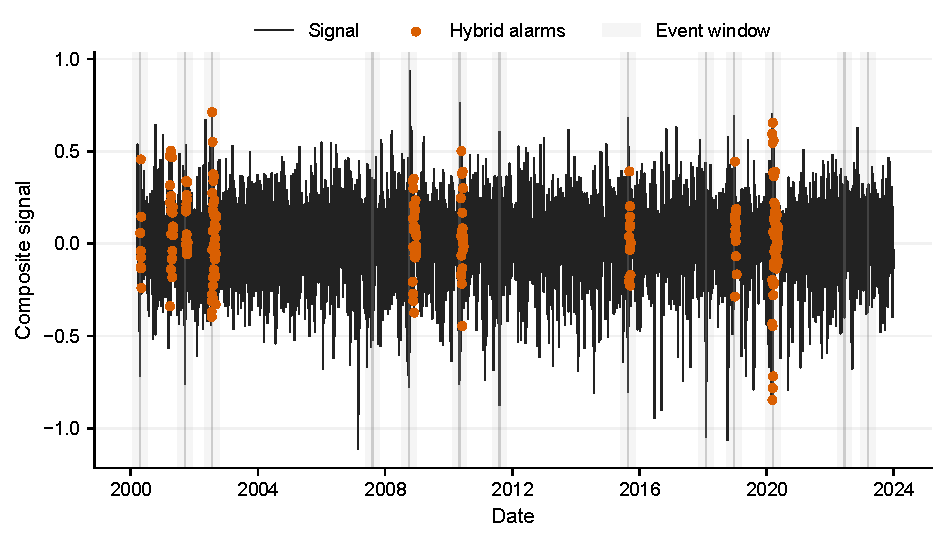
\includegraphics[width=\textwidth]{Fig1.pdf}
\caption{SPY timeline with fixed event windows and hybrid outputs, showing selective retrospective confirmation within documented stress regions.}
\label{fig:spy_timeline}
\end{figure*}


\subsection{Primary evidence: a deployed benchmark}
\label{sec:vix}
Both headline rules are constructed for this study, which invites a fair objection: perhaps the reversal is an artifact of two hand-built detectors rather than a property of the evaluation. We test that directly by running an instrument practitioners actually deploy through the identical pipeline. The Cboe Volatility Index is the market standard gauge of expected near-term equity volatility. We alarm when smoothed, calibration-standardized VIX exceeds its 90th calibration percentile, which is the same rule shape as the volatility trigger applied to a different instrument. VIX is forward looking, being priced from options, and is a level rather than a self-normalizing quantity, so it is a genuinely different signal and not a reparameterization. Table~\ref{tab:vix} reports the comparison on the SPY event panel.

\begin{table*}[t]
\centering
\caption{A deployed benchmark under the same protocol. The VIX percentile trigger and its confirmed variant are scored on the SPY event panel with identical calibration, smoothing, thresholding, and event windows. $A_{\mathrm{out}}$ counts alarm days outside all event windows; $r^{*}$ is the crossover of Equation~\eqref{eq:crossover} against the VIX trigger at $c_{\mathrm{D}}=0.05$.}
\label{tab:vix}
\begin{tabular}{lrrrrrrrr}
\toprule
Method & Precision & Recall & F1 & FPR & Events & Delay & $A_{\mathrm{out}}$ & $r^{*}$\\
\midrule
VIX percentile & 0.596 & 0.206 & 0.306 & 0.048 & 10/13 & -4.4 & 214 & \\
Volatility percentile & 0.640 & 0.225 & 0.333 & 0.044 & 10/13 & -1.2 & 195 & 0.061\\
Hybrid ($W=10$) & 0.886 & 0.122 & 0.214 & 0.005 & 8/13 & 6.8 & 24 & 0.025\\
VIX + instability confirmation & 0.947 & 0.106 & 0.190 & 0.002 & 7/13 & 3.7 & 9 & 0.022\\
\bottomrule
\end{tabular}
\end{table*}

Two results matter here. First, the protocol places the deployed benchmark sensibly: VIX detects 10 of 13 episodes, the same count as the study's volatility trigger, and fires earlier, with mean first detection at $-4.4$ trading days against $-1.2$, and a cumulative positive-delay burden of 12 trading days against 35. That is what a forward-looking instrument should do, and the delay metric registers it. The two triggers reach the same count through different episodes. VIX catches Volmageddon, which both study detectors miss and which was itself a volatility-product dislocation, while missing the dot-com selloff, where implied volatility was elevated throughout the calibration segment and so never stood out against its own history. Equal headline coverage, different events: exactly the distinction event-level scoring is designed to expose.

Second, and more important for the paper's claim, the reversal replicates on the benchmark. Gating VIX with the same instability confirmation raises precision to 0.947 and cuts FPR to 0.002, the best values anywhere in this study, and reduces out-of-window alarm days from 214 to 9. It also drops event coverage from 10 of 13 to 7 and F1 from 0.306 to 0.190. The crossover against the unconfirmed VIX trigger is 0.022, close to the 0.021 obtained for the study's own pair. The inversion is therefore not a quirk of a study-specific volatility rule. It is what confirmation does to a broad trigger under event-fixed scoring, and it appears whether the broad trigger is built for the paper or taken off the shelf.

\subsection{Primary evidence: multi-asset validation}

Table~\ref{tab:multiasset_pointwise} and Figure~\ref{fig:multiasset_tradeoff} apply the protocol to all five assets. The same tradeoff appears everywhere: lower FPR for the hybrid, lower recall and F1. Magnitudes differ. QQQ shows FPR falling from 0.039 to 0.006 while F1 falls from 0.280 to 0.139. IWM shows a smaller FPR reduction, 0.056 to 0.028, with F1 falling from 0.272 to 0.159. HYG and TLT repeat the pattern with different delay behavior, the hybrid signalling slightly earlier than volatility on HYG and later on TLT. Across the five assets this is a recurring tradeoff, not a general improvement.

\begin{table*}[t]
\centering
\caption{Multi-asset event-fixed pointwise evaluation for the volatility trigger and hybrid confirmation rule.}
\label{tab:multiasset_pointwise}
\scriptsize
\begin{tabular}{llrrrrrr}
\toprule
Ticker & Method & Precision & Recall & F1 & FPR & Mean delay & Align. err.\\
\midrule
SPY & Volatility & 0.640 & 0.225 & 0.333 & 0.044 & -1.2 & 3.6\\
SPY & Hybrid & 0.886 & 0.122 & 0.214 & 0.005 & 6.8 & 8.3\\
QQQ & Volatility & 0.616 & 0.181 & 0.280 & 0.039 & -19.3 & 3.2\\
QQQ & Hybrid & 0.812 & 0.076 & 0.139 & 0.006 & 10.4 & 15.2\\
IWM & Volatility & 0.529 & 0.183 & 0.272 & 0.056 & -0.3 & 4.4\\
IWM & Hybrid & 0.536 & 0.093 & 0.159 & 0.028 & 14.2 & 16.2\\
HYG & Volatility & 0.501 & 0.163 & 0.246 & 0.064 & 0.2 & 2.2\\
HYG & Hybrid & 0.650 & 0.110 & 0.188 & 0.024 & -1.0 & 2.3\\
TLT & Volatility & 0.507 & 0.281 & 0.362 & 0.085 & -25.3 & 4.7\\
TLT & Hybrid & 0.367 & 0.094 & 0.150 & 0.051 & -4.8 & 23.5\\
\bottomrule
\end{tabular}
\end{table*}

\begin{figure*}[t]
\centering
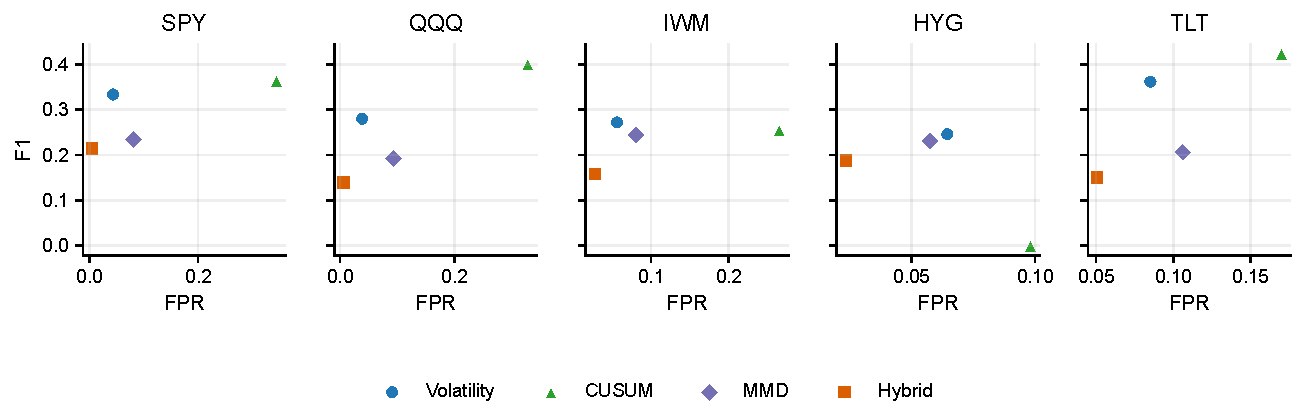
\includegraphics[width=\textwidth]{Fig2.pdf}
\caption{Multi-asset FPR--F1 tradeoff under the common event-fixed protocol without asset-specific detector tuning.}
\label{fig:multiasset_tradeoff}
\end{figure*}

\subsection{Primary evidence: event-level analysis}
Pointwise recall and FPR cannot say whether an individual stress episode was caught at all. Table~\ref{tab:spy_event_level} and Figure~\ref{fig:event_level_delay} give the SPY event-level comparison. The hybrid detects 8 of 13 events against 10 of 13 for volatility. It misses the U.S. downgrade and the 2022 inflation selloff, both of which volatility catches. Both methods miss the quant crisis, Volmageddon, and the 2023 bank stress episode under the fixed $\pm60$-day window. Among detected events the hybrid usually covers less of the window, with equal or later first detection. Lehman is the extreme case at $+33$ trading days against $-7$ for volatility, a gap of 40 trading days on the single most severe episode in the panel.

\begin{table*}[t]
\centering
\caption{SPY event-level detection, FDD, and event-window coverage for volatility and hybrid outputs.}
\label{tab:spy_event_level}
\scriptsize
\begin{tabular}{llrrrrrr}
\toprule
Event & Severity & Vol. det. & Hyb. det. & Vol. delay & Hyb. delay & Vol. cov. & Hyb. cov.\\
\midrule
Dot-com selloff & high & 1 & 1 & 4 & 4 & 0.241 & 0.096\\
September 11 reopening & critical & 1 & 1 & 6 & 6 & 0.132 & 0.124\\
WorldCom selloff & critical & 1 & 1 & -8 & -4 & 0.446 & 0.306\\
Quant crisis & medium & 0 & 0 & NA & NA & 0.000 & 0.000\\
Lehman crisis & critical & 1 & 1 & -7 & 33 & 0.562 & 0.231\\
Flash crash & high & 1 & 1 & 11 & 11 & 0.174 & 0.174\\
U.S. downgrade & critical & 1 & 0 & 2 & NA & 0.405 & 0.000\\
China devaluation & medium & 1 & 1 & 8 & 8 & 0.116 & 0.116\\
Volmageddon & medium & 0 & 0 & NA & NA & 0.000 & 0.000\\
Q4 2018 selloff & high & 1 & 1 & 4 & 4 & 0.124 & 0.124\\
COVID crash & critical & 1 & 1 & -8 & -8 & 0.405 & 0.405\\
Inflation selloff & high & 1 & 0 & -24 & NA & 0.331 & 0.000\\
Bank stress & medium & 0 & 0 & NA & NA & 0.000 & 0.000\\
\bottomrule
\end{tabular}
\end{table*}

\subsubsection{Why the hybrid misses what it misses}
\label{sec:mechanism}
Table~\ref{tab:spy_event_level} is usually read as a scoreboard. Read as a diagnostic it identifies which component fails, and the answer is specific. Table~\ref{tab:mechanism} decomposes each event window into volatility alarm days, instability alarm days, and the peak smoothed $z_{\mathrm{MMD}}$ reached inside the window.

\begin{table*}[t]
\centering
\caption{Component diagnosis per SPY event window ($\pm60$ trading days, 121 days per window). Volatility and instability alarm days are counted inside the window; peak $z_{\mathrm{MMD}}$ is the maximum smoothed standardized MMD attained there.}
\label{tab:mechanism}
\scriptsize
\begin{tabular}{lrrrrr}
\toprule
Event & Vol. det. & Hyb. det. & Vol. alarm days & Instab. alarm days & Peak $z_{\mathrm{MMD}}$\\
\midrule
Dot-com selloff & 1 & 1 & 20 & 21 & 4.39\\
September 11 reopening & 1 & 1 & 16 & 20 & 1.79\\
WorldCom selloff & 1 & 1 & 54 & 17 & 2.14\\
Quant crisis & 0 & 0 & 0 & 24 & 2.71\\
Lehman crisis & 1 & 1 & 68 & 10 & 2.15\\
Flash crash & 1 & 1 & 21 & 49 & 4.88\\
U.S. downgrade & 1 & 0 & 49 & 1 & 0.96\\
China devaluation & 1 & 1 & 14 & 44 & 2.44\\
Volmageddon & 0 & 0 & 0 & 7 & 1.62\\
Q4 2018 selloff & 1 & 1 & 15 & 17 & 2.65\\
COVID crash & 1 & 1 & 49 & 46 & 6.56\\
Inflation selloff & 1 & 0 & 40 & 2 & 1.84\\
Bank stress & 0 & 0 & 0 & 0 & 0.14\\
\bottomrule
\end{tabular}
\end{table*}

The two events the hybrid alone misses are not near misses. On the U.S. downgrade, volatility is active on 49 of 121 window days and instability on 1. On the inflation selloff the counts are 40 and 2. Across the eight events the hybrid does confirm, instability is active on between 10 and 49 window days, mean 28.0. The confirmation gate did not narrowly fail on these two episodes. It never opened.

Nor is the volatility component at fault. It was firing steadily through both windows. What failed is the kernel statistic that drives confirmation: peak $z_{\mathrm{MMD}}$ reaches only 0.96 and 1.84, against a mean of 3.38 across confirmed events.

The reason traces back to the composite signal. Because $x_t$ is effectively a standardized return, and standardization divides by a trailing 50-day standard deviation, a volatility increase that the trailing window can absorb produces no lasting change in the distribution of $x_t$. Measuring dispersion inside each $\pm60$ window against the 120 trading days preceding it makes the compression visible. Across the seven confirmed events with a full pre-window available, the dispersion of raw volatility rises by a factor of 3.03 while the dispersion of $x_t$ rises by 1.29. The U.S. downgrade is the clean illustration: raw volatility dispersion rises 3.26 times, the composite only 1.24, and $z_{\mathrm{MMD}}$ never clears 1. The 2022 inflation selloff is the other variety, a grinding repricing in an already-unsettled year, where raw volatility dispersion rises just 1.11 and the composite dispersion actually falls to 0.85.

Two clarifications keep this claim honest. First, this is not a story about speed. The events the hybrid misses have shorter peak-to-trough spans on average, 13.2 trading days against 22.5 for confirmed events, so a simple gradual-versus-abrupt reading fails. Second, it is not purely a story about size, though realized severity does separate the groups on average, 0.196 against 0.110. The U.S. downgrade carries a 0.166 drawdown and a 6.73\% worst day, larger than six of the eight confirmed events, and is still missed.

What survives both checks is scale contrast. The hybrid confirms an episode when returns move faster than the trailing 50-day scale can adapt, and stays silent when the scale keeps up, however elevated the resulting volatility. That makes the two detectors non-nested in a way F1 conceals. One reads the level of volatility, the other reads change in a self-normalizing signal. The confirmation layer is not a stricter volatility trigger; it answers a different question. Any confirmation rule built on standardized inputs will inherit this blind spot, which is a design lesson rather than a property of this particular threshold. Because this reading rests on only two missed events, Section~\ref{sec:mechtest} tests it under controlled synthetic conditions, where both directions of the prediction can be engineered.

\subsubsection{A controlled synthetic test of the mechanism}
\label{sec:mechtest}
Two missed events are thin evidence, however consistent. The mechanism makes a prediction sharp enough to test under controlled conditions, so we test it. We generate a Gaussian return series and run the paper's exact preprocessing, calibration, thresholds, and confirmation pipeline on it. The series contains two engineered stress episodes with the same peak volatility, three times baseline (Figure~\ref{fig:mechtest}). Episode A is an abrupt break: volatility jumps to its peak overnight and holds for 60 days, faster than the trailing 50-day standardization scale can adapt. Episode B is an absorbed ramp: volatility climbs to the same peak and back down along a symmetric 300-day triangle, with no jump at either edge, slowly enough for the trailing scale to track it. A third abrupt episode placed inside the calibration segment gives the 90th-percentile thresholds the same crisis-contaminated training that the SPY calibration period has.

The prediction holds in both directions. The volatility trigger fires through both episodes, on 54 of 60 days in A and 254 of 300 in B: the raw scale sees both. The kernel gate separates them. MMD-only confirmation fires on 36 of 60 days in A (60\%) against 9 of 300 in B (3\%), and peak smoothed $z_{\mathrm{MMD}}$ reaches 4.95 in A against 1.79 in B. A 90th-percentile threshold fires on 10\% of calibration days by construction, so the absorbed ramp sits below the base rate while the abrupt break sits six times above it. The full instability score shows the same contrast, 57\% against 7\%, and the residual firing inside B traces to the two-sided $\kappa$ noise term rather than to the kernel statistic. An episode the trailing scale can absorb is invisible to the confirmation layer even at three times baseline volatility, exactly as the construction of $x_t$ implies. One scope note: the synthetic operationalizes absorption through the ramp mode, and neither engineered episode replicates the two SPY misses, one a sharp expansion the trailing window caught up to within its 50-day span, the other an episode inside a regime whose elevated scale was already in the denominator. Both are variants of the same scale mechanism, and the test demonstrates that mechanism, not the individual cases.


The multi-asset event-level summary in Table~\ref{tab:multiasset_event_level} repeats the pattern. Hybrid detection rates trail volatility on every asset: 0.615 against 0.769 on SPY, 0.385 against 0.462 on QQQ, 0.385 against 0.538 on IWM, 0.231 against 0.385 on HYG, and 0.308 against 0.538 on TLT. Mean coverage is lower everywhere. Median FDD is later on SPY, QQQ, IWM, and TLT, with HYG again the exception.

One accounting choice in these rates needs to be stated plainly. Every rate in Table~\ref{tab:multiasset_event_level} uses all 13 events as its denominator, but IWM begins trading in August 2000, TLT in October 2002, and HYG in June 2007, so some panel events predate the asset entirely. The calendar-to-trading-day mapping sends a pre-inception event to the asset's earliest available date, which stacks one degenerate window at the start of the IWM series and three each for HYG and TLT. No degenerate window is detected by either method, so the level of the HYG and TLT rates is pulled down by construction. Restated over the events each asset can actually observe, the rates are 7 of 12 against 5 of 12 for IWM, 5 of 10 against 3 of 10 for HYG, and 7 of 10 against 4 of 10 for TLT, volatility first in each pair. The within-asset comparison is unaffected, because both detectors face the same available events, but cross-asset comparisons of detection level should use the restated figures.

To be explicit about propagation: every computation in the paper uses all 13 mapped windows, degenerate ones included. The cost and crossover comparisons are insensitive to this choice, because both detectors miss every degenerate window, so the missed-event differences entering Equation~\eqref{eq:crossover} are identical either way (2 for HYG and 3 for TLT, with or without the degenerate events) and no delay terms arise from undetected events. Pointwise metrics do include the degenerate windows in the positive mask, which adds a stretch of positive-class days at the start of the affected series; this affects both detectors identically and merges with the earliest observable event's window where the two overlap, as they do for HYG.

\begin{table*}[t]
\centering
\caption{Multi-asset event-level detection rate, median delay, and mean event-window coverage. All rates use the full 13-event panel as denominator; rates restated over each asset's observable events are given in the text.}
\label{tab:multiasset_event_level}
\scriptsize
\begin{tabular}{llrrr}
\toprule
Ticker & Method & Detect. rate & Med. delay & Mean cov.\\
\midrule
SPY & Vol. & 0.769 & 3.0 & 0.226\\
SPY & Hybrid & 0.615 & 5.0 & 0.121\\
QQQ & Vol. & 0.462 & -11.5 & 0.198\\
QQQ & Hybrid & 0.385 & 2.0 & 0.086\\
IWM & Vol. & 0.538 & 1.0 & 0.176\\
IWM & Hybrid & 0.385 & 5.0 & 0.090\\
HYG & Vol. & 0.385 & 2.0 & 0.123\\
HYG & Hybrid & 0.231 & -3.0 & 0.083\\
TLT & Vol. & 0.538 & -4.0 & 0.227\\
TLT & Hybrid & 0.308 & -2.5 & 0.076\\
\bottomrule
\end{tabular}
\end{table*}

Severity-stratified results in Table~\ref{tab:event_level_severity} line up with the mechanism. Hybrid detection falls from 0.680 on critical events to 0.300 on high and 0.100 on medium, a steeper gradient than volatility's 0.840, 0.550, 0.150. The confirmation gate behaves as an implicit severity filter, which is what a rule keyed to scale contrast should do. With 13 events split into terciles these are descriptive summaries, not severity effects estimated with any precision.

\begin{table*}[t]
\centering
\caption{Severity-stratified event-level summary using descriptive realized-drawdown terciles from the SPY event panel.}
\label{tab:event_level_severity}
\scriptsize
\begin{tabular}{llrrr}
\toprule
Severity & Method & Detect. rate & Med. delay & Mean cov.\\
\midrule
Critical & Vol. & 0.840 & -2.6 & 0.317\\
Critical & Hybrid & 0.680 & 2.0 & 0.176\\
High & Vol. & 0.550 & -8.9 & 0.175\\
High & Hybrid & 0.300 & -1.3 & 0.066\\
Medium & Vol. & 0.150 & -26.0 & 0.046\\
Medium & Hybrid & 0.100 & -26.0 & 0.011\\
\bottomrule
\end{tabular}
\end{table*}

\begin{figure*}[t]
\centering
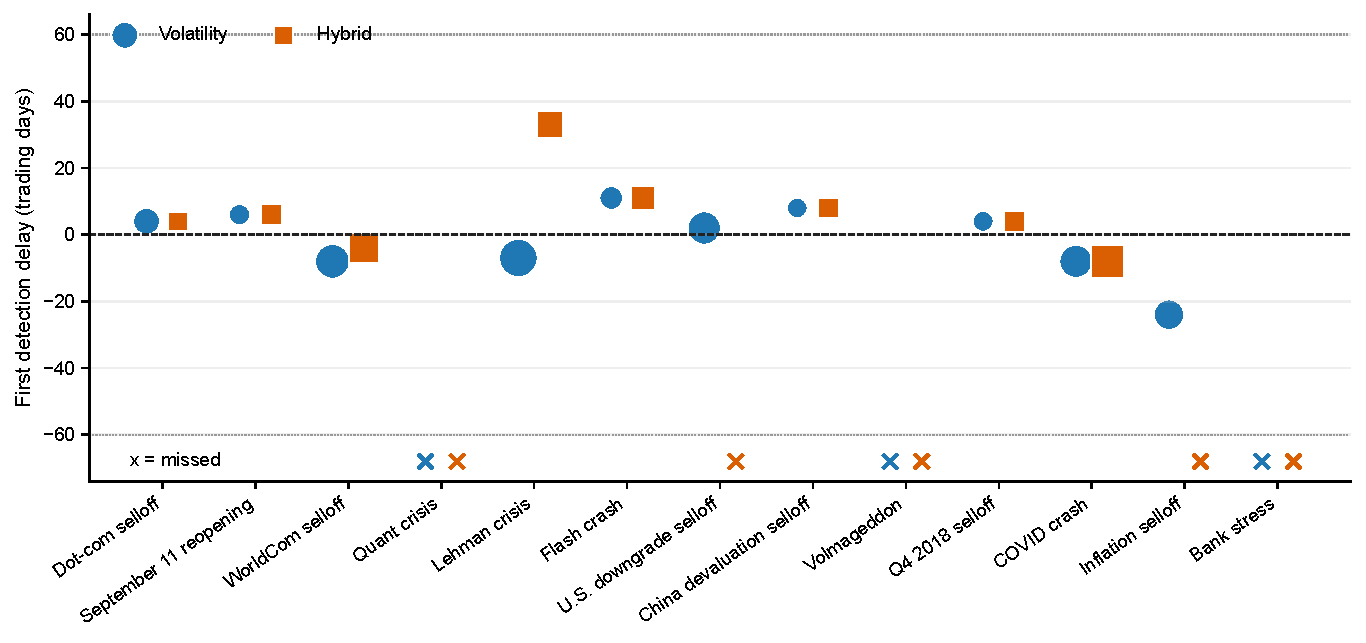
\includegraphics[width=0.95\textwidth]{Fig3.pdf}
\caption{SPY event-level FDD and event-window coverage, with missed events marked explicitly.}
\label{fig:event_level_delay}
\end{figure*}

\begin{figure*}[t]
\centering
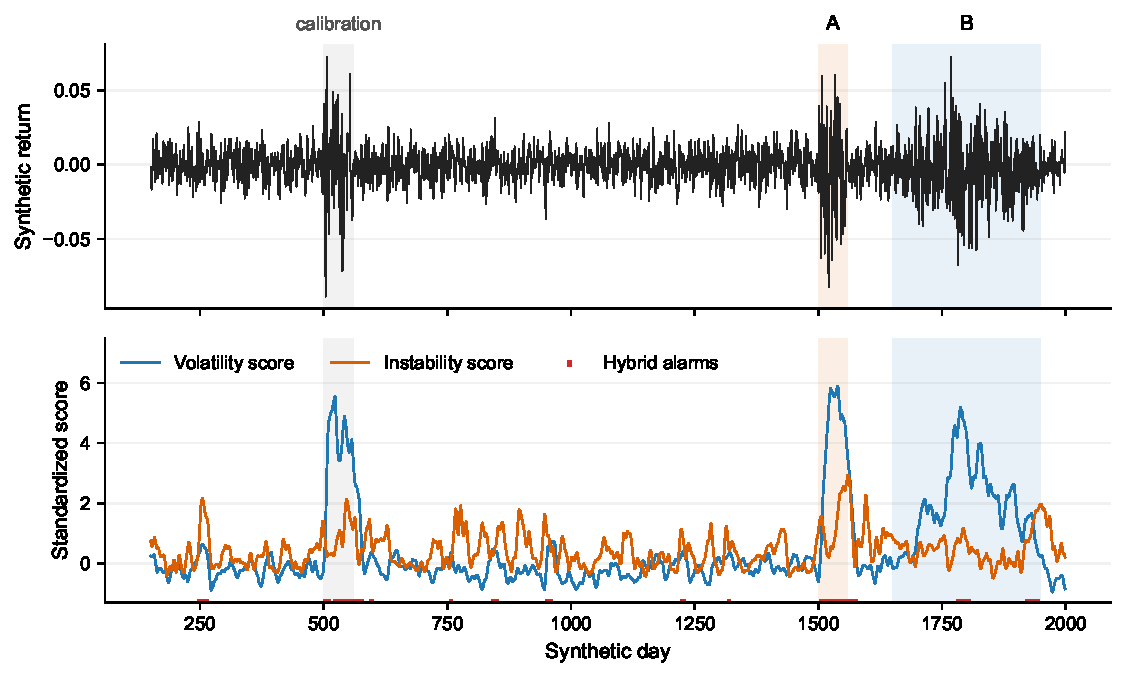
\includegraphics[width=0.9\textwidth]{Fig4.pdf}
\caption{Controlled synthetic test of the scale-adaptation mechanism. Top: a Gaussian return series with an abrupt volatility break (A) and an absorbed triangle ramp (B) of identical peak volatility, plus the abrupt calibration episode. Bottom: standardized volatility and instability scores with hybrid alarms. The volatility score rises through both episodes; the instability score responds only to the abrupt break.}
\label{fig:mechtest}
\end{figure*}

\subsection{Primary evidence: cost-sensitive interpretation}
\label{sec:cost}
A pointwise cost model shows why the precision and FPR gap matters operationally. With $c_{\mathrm{FN}}=1$ and $c_{\mathrm{FP}}/c_{\mathrm{FN}}\in\{1,2,5,10,20,50\}$, Table~\ref{tab:cost} and Figure~\ref{fig:cost} put the hybrid ahead at every tested ratio on SPY. Its margin is slim under equal weighting and widens as false positives get expensive. The pointwise mask is mostly non-event days, so cutting false positives dominates this objective even when recall, event detection, and timeliness are all worse. That is the measurement artifact the event-aware cost is designed to expose.

\begin{table}[t]
\centering
\caption{Pointwise cost-sensitive comparison with $c_{\mathrm{FN}}=1$.}
\label{tab:cost}
\scriptsize
\begin{tabular}{rrrr}
\toprule
$c_{\mathrm{FP}}/c_{\mathrm{FN}}$ & Vol. cost & Hybrid cost & Preferred\\
\midrule
1 & 1384 & 1372 & Hybrid\\
2 & 1579 & 1396 & Hybrid\\
5 & 2164 & 1468 & Hybrid\\
10 & 3139 & 1588 & Hybrid\\
20 & 5089 & 1828 & Hybrid\\
50 & 10939 & 2548 & Hybrid\\
\bottomrule
\end{tabular}
\end{table}

The event-aware results in Table~\ref{tab:event_cost} reverse the verdict at the low end. With $c_{\mathrm{ME}}=1$ and $c_{\mathrm{D}}=0.05$, volatility costs 6.70 against 8.54 for the hybrid when false-alarm days are nearly free at $c_{\mathrm{FA}}/c_{\mathrm{ME}}=0.01$. Volatility misses 3 events rather than 5 and carries a smaller cumulative delay penalty, $D_+=35$ against 66. From 0.05 upward the hybrid wins, on the strength of 24 out-of-window alarm days against 195.

\begin{table*}[t]
\centering
\caption{SPY event-aware cost comparison with $c_{\mathrm{ME}}=1$ and $c_{\mathrm{D}}=0.05$.}
\label{tab:event_cost}
\scriptsize
\begin{tabular}{lrrrr}
\toprule
$c_{\mathrm{FA}}/c_{\mathrm{ME}}$ & Vol. cost & Hybrid cost & Vol. missed & Hyb. missed\\
\midrule
0.01 & 6.70 & 8.54 & 3 & 5\\
0.05 & 14.50 & 9.50 & 3 & 5\\
0.10 & 24.25 & 10.70 & 3 & 5\\
0.25 & 53.50 & 14.30 & 3 & 5\\
0.50 & 102.25 & 20.30 & 3 & 5\\
1.00 & 199.75 & 32.30 & 3 & 5\\
\bottomrule
\end{tabular}
\end{table*}

\subsubsection{The crossover ratio}
Reporting that the answer depends on the cost structure is not useful to anyone who has to choose. The crossover is computable. Equation~\eqref{eq:eventcost} is linear in $c_{\mathrm{FA}}$, so setting $C_{\mathrm{event}}^{\mathrm{vol}}=C_{\mathrm{event}}^{\mathrm{hyb}}$ and solving gives
\begin{equation}
\label{eq:crossover}
r^{*}=\frac{(M_{\mathrm{hyb}}-M_{\mathrm{vol}})+c_{\mathrm{D}}(D_{+}^{\mathrm{hyb}}-D_{+}^{\mathrm{vol}})}{A_{\mathrm{out}}^{\mathrm{vol}}-A_{\mathrm{out}}^{\mathrm{hyb}}},
\end{equation}
with the volatility trigger preferred below $r^{*}$ and the hybrid above it, whenever the hybrid raises fewer out-of-window alarms. Substituting the SPY values from Table~\ref{tab:event_cost} at $c_{\mathrm{D}}=0.05$, namely $M=3$ and $5$, $D_+=35$ and $66$, and $A_{\mathrm{out}}=195$ and $24$,
\begin{equation}
r^{*}=\frac{(5-3)+0.05(66-35)}{195-24}=\frac{3.55}{171}=0.021 .
\end{equation}

So the volatility trigger is the cheaper choice on SPY only when one out-of-window alarm day costs less than 0.021 of a missed stress episode. Inverted, a missed episode must be worth more than 48 false alarm days for volatility to win. A desk triaging one alerting day per analyst-hour should prefer the volatility trigger if it values a missed episode above roughly 48 analyst-hours of review, and the hybrid otherwise. The tested grid straddles this point, which is why the preference flips between 0.01 and 0.05. Readers who know the early-warning literature will recognize $r^{*}$ as a delay-aware, asymmetric cousin of the noise-to-signal ratio \cite{kaminsky1998}: both compress the false-alarm-versus-missed-crisis tradeoff into one number, but $r^{*}$ prices delay and lets the two error types carry different weights.

Table~\ref{tab:crossover} gives $r^{*}$ for all five assets and all three delay penalties. Every value falls between 0.007 and 0.059, so the region favouring volatility is narrow throughout: out-of-window alarms have to be very cheap relative to missed episodes before broad coverage pays. Raising $c_{\mathrm{D}}$ widens that region on four assets, because the hybrid confirms later and absorbs more delay penalty. HYG moves the other way, from 0.016 to 0.013, and the reason is visible in Table~\ref{tab:multiasset_event_level}: HYG is the one asset where the hybrid detects earlier than volatility, so penalizing delay works in its favour.

\begin{table}[t]
\centering
\caption{Event-aware cost crossover ratio $r^{*}=c_{\mathrm{FA}}/c_{\mathrm{ME}}$ from Equation~\eqref{eq:crossover}. Below $r^{*}$ the volatility trigger has lower cost; above it the hybrid does.}
\label{tab:crossover}
\scriptsize
\begin{tabular}{lrrr}
\toprule
Ticker & $c_{\mathrm{D}}=0$ & $c_{\mathrm{D}}=0.05$ & $c_{\mathrm{D}}=0.1$\\
\midrule
SPY & 0.012 & 0.021 & 0.030\\
QQQ & 0.007 & 0.027 & 0.047\\
IWM & 0.016 & 0.038 & 0.059\\
HYG & 0.016 & 0.015 & 0.013\\
TLT & 0.021 & 0.034 & 0.047\\
\bottomrule
\end{tabular}
\end{table}

\begin{figure*}[t]
\centering
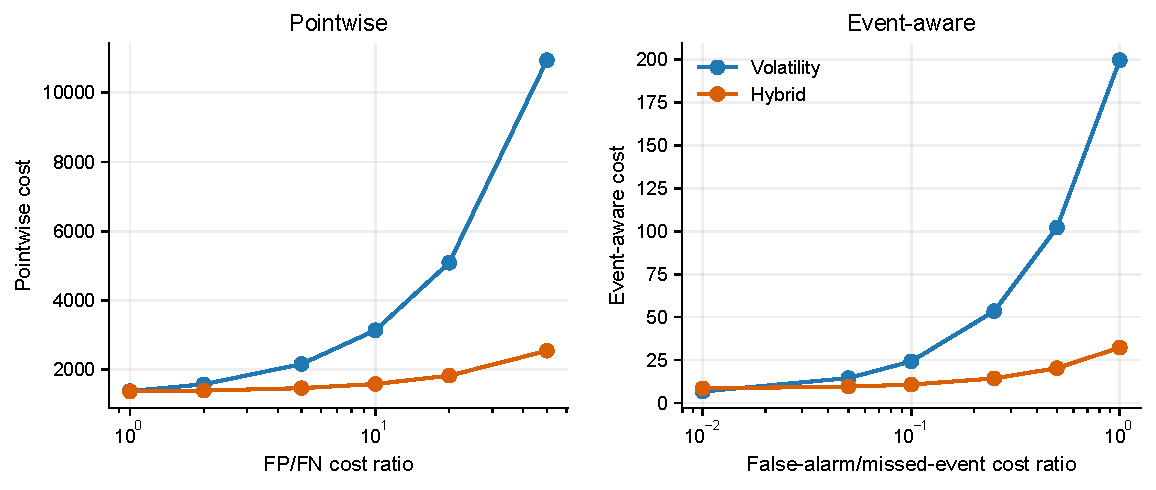
\includegraphics[width=0.95\textwidth]{Fig5.pdf}
\caption{SPY cost comparison under pointwise and event-aware operating objectives.}
\label{fig:cost}
\end{figure*}

\subsection{Secondary robustness: event-window sensitivity}
Table~\ref{tab:eventwindow} and Figure~\ref{fig:eventwindow} show the tradeoff holding across window widths. The hybrid keeps lower FPR and higher precision, with lower recall and F1, at every width tested. The gap widens as windows lengthen, since wider windows admit more of the volatility trigger's in-window alarms.

\begin{table*}[t]
\centering
\caption{Event-window sensitivity for pointwise precision, recall, F1, and FPR.}
\label{tab:eventwindow}
\scriptsize
\begin{tabular}{llrrrr}
\toprule
Window & Method & Prec. & Recall & F1 & FPR\\
\midrule
$\pm20$ & Vol. & 0.390 & 0.396 & 0.393 & 0.061\\
$\pm20$ & Hybrid & 0.545 & 0.216 & 0.309 & 0.018\\
$\pm30$ & Vol. & 0.499 & 0.344 & 0.407 & 0.052\\
$\pm30$ & Hybrid & 0.692 & 0.186 & 0.293 & 0.012\\
$\pm45$ & Vol. & 0.571 & 0.266 & 0.363 & 0.048\\
$\pm45$ & Hybrid & 0.815 & 0.148 & 0.251 & 0.008\\
$\pm60$ & Vol. & 0.640 & 0.225 & 0.333 & 0.044\\
$\pm60$ & Hybrid & 0.886 & 0.122 & 0.214 & 0.005\\
\bottomrule
\end{tabular}
\end{table*}

\begin{figure*}[t]
\centering
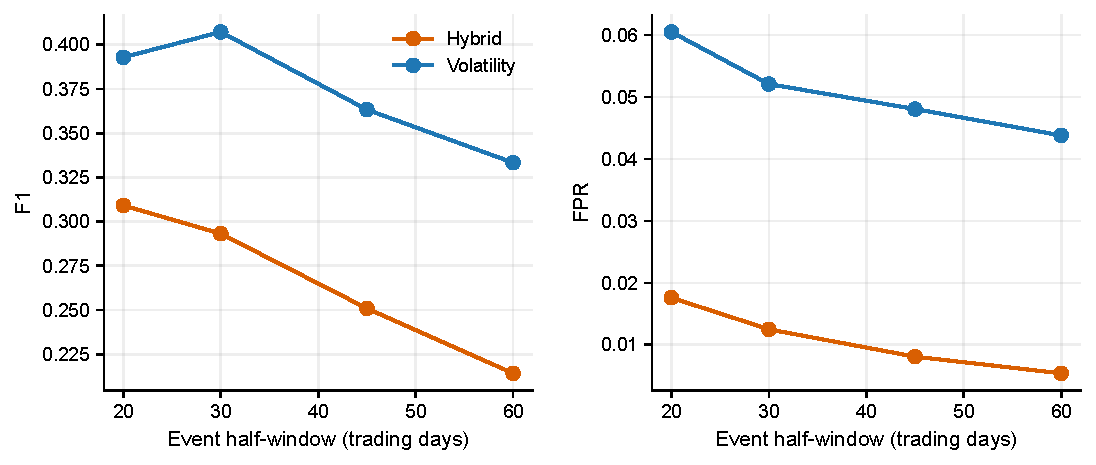
\includegraphics[width=\textwidth]{Fig6.pdf}
\caption{Event-window sensitivity across $\pm20$, $\pm30$, $\pm45$, and $\pm60$ trading-day windows.}
\label{fig:eventwindow}
\end{figure*}

\subsection{Secondary robustness: composite signal weights}
\label{sec:weights}
The weights $(0.5,0.3,0.2)$ are heuristic, so their influence should be measured rather than asserted. Table~\ref{tab:weights} re-runs the full pipeline under ten weightings, recomputing the composite, MMD, $\kappa$, the instability score, and the hybrid each time. The volatility trigger is untouched, since it reads $\sigma_t$ directly.

\begin{table*}[t]
\centering
\caption{Composite weight ablation. Each row recomputes $x_t$, the MMD and $\kappa$ components, and the hybrid. Events are counted out of 13.}
\label{tab:weights}
\scriptsize
\begin{tabular}{lrrrrrr}
\toprule
$(w_r,w_\sigma,w_z)$ & Prec. & Recall & F1 & FPR & Delay & Events\\
\midrule
$(0.5,0.3,0.2)$ default & 0.886 & 0.122 & 0.214 & 0.005 & 6.8 & 8\\
$(1/3,1/3,1/3)$ equal & 0.886 & 0.122 & 0.214 & 0.005 & 6.8 & 8\\
$(0.2,0.3,0.5)$ reversed & 0.886 & 0.122 & 0.214 & 0.005 & 6.8 & 8\\
$(0.6,0.2,0.2)$ & 0.882 & 0.122 & 0.214 & 0.006 & 6.8 & 8\\
$(0.4,0.4,0.2)$ & 0.886 & 0.122 & 0.214 & 0.005 & 6.8 & 8\\
$(0.5,0.2,0.3)$ & 0.886 & 0.122 & 0.214 & 0.005 & 6.8 & 8\\
$(0.2,0.6,0.2)$ & 0.900 & 0.135 & 0.235 & 0.005 & 4.4 & 8\\
$(1,0,0)$ returns only & 0.845 & 0.131 & 0.227 & 0.008 & 0.8 & 8\\
$(0,1,0)$ volatility only & 0.815 & 0.121 & 0.210 & 0.009 & 1.4 & 7\\
$(0,0,1)$ z-score only & 0.886 & 0.122 & 0.214 & 0.005 & 6.8 & 8\\
\bottomrule
\end{tabular}
\end{table*}

Hybrid F1 spans $[0.210,0.235]$ and FPR spans $[0.005,0.009]$ across all ten. Event detection is 8 of 13 in nine cases and 7 in the tenth. Every configuration stays far from the volatility trigger's F1 of 0.333, FPR of 0.044, and 10 of 13 events, so the ranking reversal is a property of the confirmation structure and not of the weighting.

Four rows are numerically identical, including the default, the equal weighting, the reversed weighting, and the $z$-score-only case. That is the scale argument from the preprocessing section showing up in the output: once $z_t$ carries a standard deviation two orders of magnitude above the other terms, redistributing weight among them changes nothing the kernel can detect. The two rows that do move are the ones that remove $z_t$ entirely. Dropping to volatility alone costs an event and lifts FPR to 0.009; returns alone pulls mean delay down to $+0.8$ days, the earliest confirmation in the table, at the cost of precision. Reporting the composite as a weighted blend of three inputs overstates what the weights do, and we prefer to say so plainly.

\subsection{Secondary robustness: sign convention for $\kappa$}
\label{sec:kappasign}
Table~\ref{tab:kappasign} compares the two-sided statistic against both one-sided alternatives.

\begin{table*}[t]
\centering
\caption{Confirmation-term ablation for the persistence statistic. The low-$\kappa$ variant is the direction predicted by critical-slowing-down theory.}
\label{tab:kappasign}
\scriptsize
\begin{tabular}{lrrrrrr}
\toprule
Confirmation term & Prec. & Recall & F1 & FPR & Delay & Events\\
\midrule
$|z_\kappa|$ two-sided (default) & 0.886 & 0.122 & 0.214 & 0.005 & 6.8 & 8\\
$\max(-z_\kappa,0)$ low $\kappa$ & 0.875 & 0.114 & 0.202 & 0.006 & 6.7 & 7\\
$\max(+z_\kappa,0)$ high $\kappa$ & 0.874 & 0.141 & 0.242 & 0.007 & 1.6 & 7\\
\bottomrule
\end{tabular}
\end{table*}

Restricting to the theory-consistent low-$\kappa$ direction detects 7 events rather than 8 and lowers F1 to 0.202. The opposite restriction raises F1 to 0.242 but also detects 7, and it confirms much earlier at $+1.6$ days. All three variants stay well inside the band the weight ablation traces out, so the conclusions do not turn on this convention either. We keep the two-sided form, and the sign-convention discussion in the detector definitions states plainly that it is an abnormal-dependence criterion rather than a test of critical slowing down.

\subsection{Secondary robustness: from retrospective to causal confirmation}
\label{sec:causal}
The default hybrid looks ahead in two places: the symmetric $\pm W$ confirmation window, and the MMD statistic itself, whose post-window covers $x_{t:t+29}$. A reader can fairly ask whether the reversal is an artifact of that hindsight. Table~\ref{tab:causal} answers by removing the look-ahead in stages on SPY.

\begin{table*}[t]
\centering
\caption{From retrospective to causal confirmation on SPY. Trailing variants replace the symmetric window $[t-W,t+W]$ with $[t-W,t]$; fully causal variants additionally lag the MMD component by its 30-day post-window so no input uses future data. $r^{*}$ is the crossover of Equation~\eqref{eq:crossover} at $c_{\mathrm{D}}=0.05$.}
\label{tab:causal}
\scriptsize
\begin{tabular}{lrrrrrrrr}
\toprule
Variant & Prec. & Recall & F1 & FPR & Events & Delay & $A_{\mathrm{out}}$ & $r^{*}$\\
\midrule
Symmetric $W=10$ (default) & 0.886 & 0.122 & 0.214 & 0.005 & 8/13 & 6.8 & 24 & 0.021\\
Trailing $W=10$ & 0.917 & 0.100 & 0.181 & 0.003 & 8/13 & 10.8 & 14 & 0.027\\
Trailing $W=20$ & 0.838 & 0.115 & 0.202 & 0.008 & 8/13 & 9.5 & 34 & 0.028\\
Fully causal, $W=10$ & 0.659 & 0.058 & 0.107 & 0.010 & 4/13 & 15.8 & 46 & 0.051\\
Fully causal, $W=40$ & 0.568 & 0.090 & 0.155 & 0.024 & 7/13 & 10.3 & 105 & 0.058\\
Volatility (reference) & 0.640 & 0.225 & 0.333 & 0.044 & 10/13 & -1.2 & 195 & \\
\bottomrule
\end{tabular}
\end{table*}

The first stage removes the decision-rule look-ahead but not the statistic's, and the reversal survives it cleanly. A trailing $W=10$ confirmation detects the same 8 events as the symmetric rule, sharpens precision to 0.917, and cuts out-of-window alarm days from 24 to 14, against lower recall and a later mean first detection of $+10.8$ days. The price of causality is paid where the symmetric window had been borrowing from the future: WorldCom moves from $-4$ to $+6$, the Flash Crash from $+11$ to $+21$, and Lehman from $+33$ to $+43$ trading days. Every conclusion in the paper, including the sign of the ranking reversal and a crossover ratio near 0.03, carries over to this variant unchanged.

The second stage is more revealing. Lagging the MMD component by its own 30-day post-window makes the whole pipeline causal end to end, and performance drops hard: 4 of 13 events at $W=10$. Recovering coverage requires stretching the trailing window to $W=40$, which restores 7 of 13 but returns 105 out-of-window alarm days, giving back more than half of the false-alarm advantage over the volatility trigger. Most of the confirmation layer's power therefore lives in the MMD post-window, not in the symmetric confirmation window. A deployable confirmation layer of this design either waits roughly the MMD window length after the stress date or cedes much of its selectivity. The crossover ratios move accordingly, from 0.021 to at most 0.058, so the decision rule of Section~\ref{sec:cost} keeps its form in every variant, with a somewhat wider region favouring the volatility trigger as causality constraints tighten.

\subsection{Secondary robustness: severity, component, and confirmation-window analyses}
Within this panel, events in the highest realized-drawdown tercile give F1 0.412 for volatility and 0.316 for the hybrid, with FPR falling from 0.057 to 0.015. The middle tercile gives F1 0.195 against 0.134 and FPR 0.080 against 0.030. The lowest tercile gives very low F1 for both.

The MMD-only row in Table~\ref{tab:spy} is the standalone thresholded MMD component. The component ablation instead uses MMD-only as the confirmation signal inside the hybrid, which gives F1 0.219 against 0.214 for the default no-CIS hybrid. The no-CIS score is the more conservative of the two, FPR 0.005 against 0.011. Figure~\ref{fig:window_sensitivity} shows $W=10$ is not F1-optimal: F1 climbs to 0.291 at $W=60$ while FPR rises to 0.031. Since these use symmetric confirmation windows, read them as retrospective sensitivity analysis.

\begin{figure*}[t]
\centering
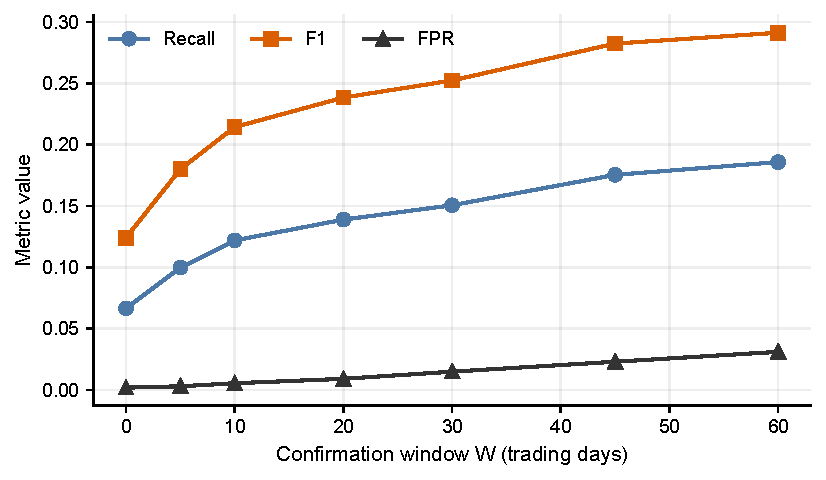
\includegraphics[width=\textwidth]{Fig7.pdf}
\caption{Hybrid confirmation-window sensitivity showing how the retrospective confirmation window changes F1 and FPR.}
\label{fig:window_sensitivity}
\end{figure*}

\subsection{Secondary robustness: bootstrap uncertainty}
\label{sec:bootstrap}
The event bootstrap gives hybrid-minus-volatility $\Delta$F1 $=-0.091$ with 95\% CI $[-0.166,0.005]$, and $\Delta$FPR $=-0.045$ with CI $[-0.058,-0.035]$. The block bootstrap gives $\Delta$F1 $=-0.120$ with CI $[-0.203,-0.047]$ and $\Delta$FPR $=-0.039$ with CI $[-0.062,-0.019]$. The FPR reduction is negative in all 2000 resamples under both schemes. The F1 reduction is negative in all 2000 block resamples but in 97.3\% of event resamples, and the event-bootstrap interval crosses zero, so the size of the F1 penalty is the less firmly established of the two. Figure~\ref{fig:bootstrap_violin} shows the distributions. With 13 fixed events, resampling cannot manufacture precision the panel does not contain, and the multi-asset results are directional evidence rather than a pooled estimate.

\begin{figure*}[t]
\centering
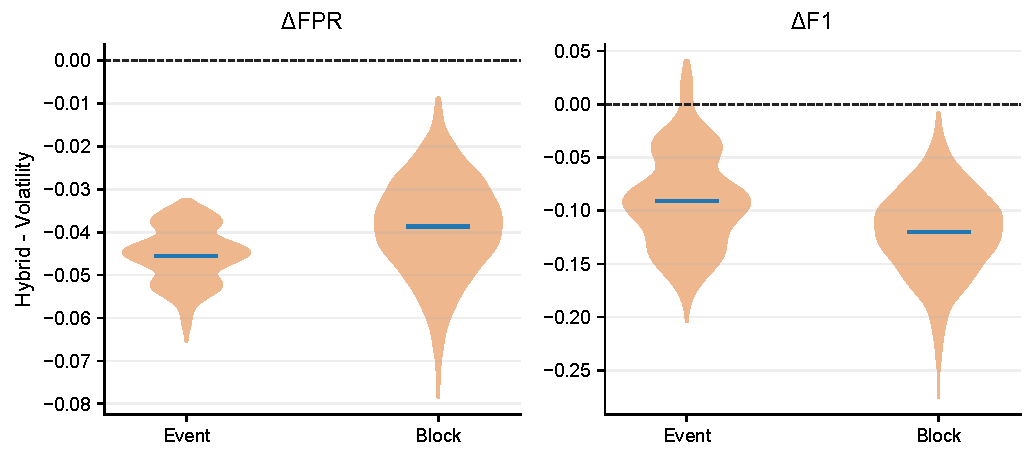
\includegraphics[width=\textwidth]{Fig8.pdf}
\caption{Bootstrap distributions of hybrid-minus-volatility differences under the fixed-event protocol.}
\label{fig:bootstrap_violin}
\end{figure*}

\subsection{Auxiliary diagnostic validation: synthetic and NAB analyses}
Figure~\ref{fig:synthetic_example} shows one generated sequence with latent labels and detector outputs.

\begin{figure*}[t]
\centering
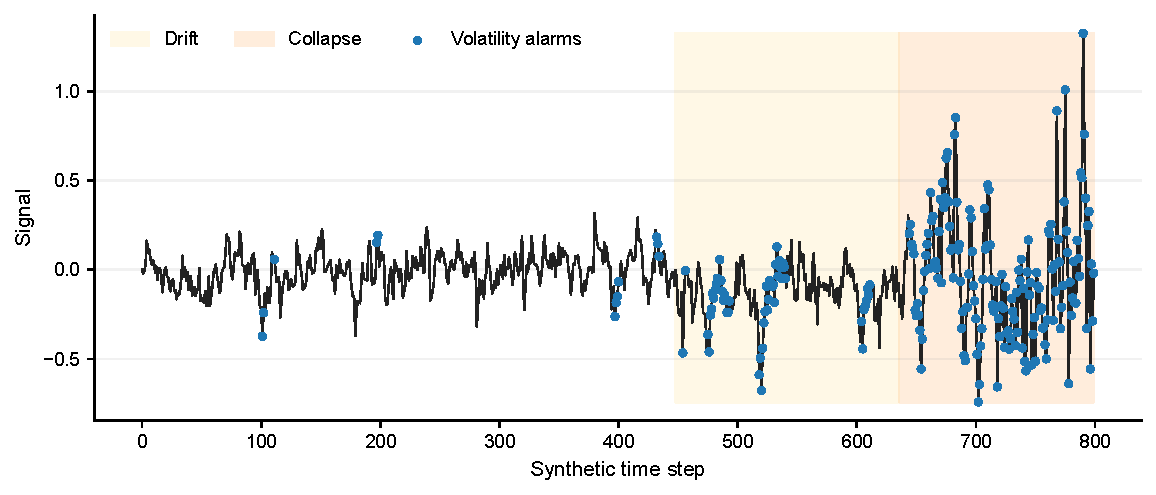
\includegraphics[width=0.95\textwidth]{Fig9.pdf}
\caption{Synthetic diagnostic validation under controlled regime changes and noisy dynamics.}
\label{fig:synthetic_example}
\end{figure*}

The synthetic example contains stable, drift, and collapse regimes with heavy-tailed noise and volatility amplification near collapse. Detector outputs track the controlled regime changes, which establishes pipeline responsiveness in the generator and nothing about real markets.

On NAB, mean F1 is nearly identical for the two rules, 0.141 for the hybrid against 0.140 for volatility, while hybrid FPR is lower at 0.105 against 0.141. That matches the SPY pattern, where confirmation cuts false positives without buying an F1 improvement. Figure~\ref{fig:nab_results} breaks this out by subset. Official NAB scores are not used, the task is not finance-specific, and the NAB path substitutes a rolling mean-difference proxy for MMD, so these are consistency checks rather than leaderboard results. Put more sharply, NAB validates the scoring harness rather than the SPY detector: with the proxy substituted for exact MMD, it is a different confirmation rule evaluated under the same metrics, so it should not be read as external replication of the hybrid.

\begin{figure*}[t]
\centering
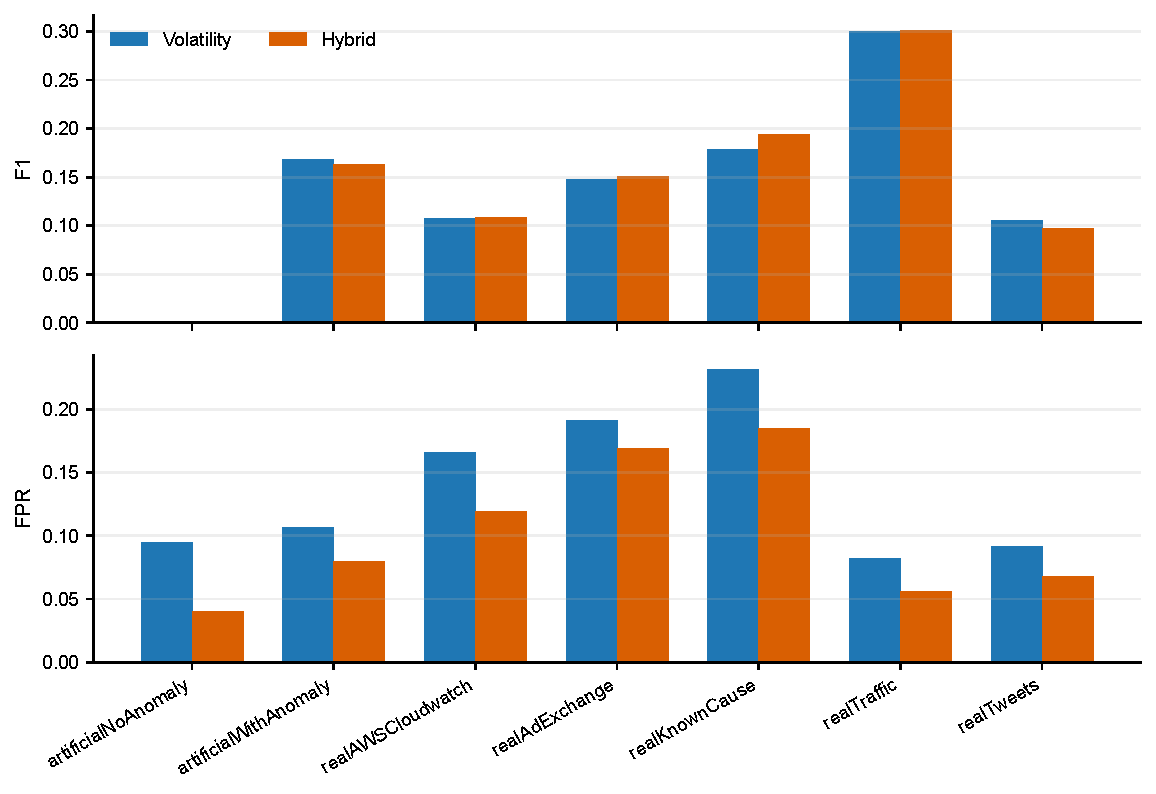
\includegraphics[width=0.95\textwidth]{Fig10.pdf}
\caption{NAB external qualitative validation by subset using the same pointwise metrics as the financial-stress protocol.}
\label{fig:nab_results}
\end{figure*}

\begin{table*}[t]
\centering
\caption{NAB subset-level F1 and FPR for volatility and hybrid outputs.}
\scriptsize
\setlength{\tabcolsep}{2pt}
\begin{tabular}{lrrrr}
\toprule
Subset & Vol. F1 & Vol. FPR & Hyb. F1 & Hyb. FPR\\
\midrule
artificialNoAnomaly & 0.000 & 0.095 & 0.000 & 0.040\\
artificialWithAnomaly & 0.168 & 0.107 & 0.163 & 0.080\\
realAWSCloudwatch & 0.108 & 0.166 & 0.108 & 0.119\\
realAdExchange & 0.148 & 0.191 & 0.151 & 0.169\\
realKnownCause & 0.179 & 0.232 & 0.194 & 0.185\\
realTraffic & 0.300 & 0.082 & 0.302 & 0.056\\
realTweets & 0.106 & 0.092 & 0.097 & 0.068\\
\bottomrule
\end{tabular}
\end{table*}

\section{Discussion}
\label{sec:discussion}
The headline result is an inversion, and it is worth stating in its sharpest form. On the same asset, over the same 24 years, from the same two output series, the hybrid is either the clearly better detector or the clearly worse one depending on whether performance is counted in alarm days or in stress events. Precision rises from 0.640 to 0.886 and FPR falls from 0.044 to 0.005. Event coverage falls from 10 of 13 to 8 of 13, recall from 0.225 to 0.122, and mean first detection slips from $-1.2$ to $+6.8$ trading days. A single F1 number hides all of this.

CUSUM makes the same point from another angle. It posts the highest F1 in Table~\ref{tab:spy} at 0.364 while running an FPR of 0.344 and a mean delay near $-60$ days, which is to say it alarms through most of the sample and gets credit for overlapping wide windows. Ranking by F1 would put it first. Ranking by precision alone would put the hybrid first by a wide margin. Both rankings are artifacts of the chosen metric.

Section~\ref{sec:mechanism} is what turns this from a scoreboard observation into something usable. The hybrid's misses are not random shortfalls in sensitivity. They are the predictable consequence of gating on a statistic whose input is self-normalizing. Because $x_t$ is effectively a standardized return, and standardization divides by a trailing 50-day scale, the MMD gate registers repricing that outruns the scale and ignores volatility that the scale has absorbed. That is why the U.S. downgrade slips through with 49 volatility alarm days and 1 instability alarm day, and why the 2022 inflation selloff slips through with 40 and 2. It also explains the severity gradient in Table~\ref{tab:event_level_severity}, where hybrid detection falls from 0.680 on critical events to 0.100 on medium ones, considerably steeper than volatility's decline.

The practical consequence is a design constraint rather than a tuning recommendation. Any confirmation layer built on standardized inputs will be blind to repricings its normalization window has already absorbed, no matter where the threshold sits, and Section~\ref{sec:mechanism} shows this is a matter of scale adaptation rather than speed: the absorbed episodes include a sharp spike the trailing window caught up to and an episode unfolding inside an already-elevated volatility regime, not the slow-moving ones. Widening the confirmation window from 10 to 60 days raises F1 to 0.291 but also lifts FPR to 0.031 and does not address the normalization. Institutions that need to flag stress the trailing scale has absorbed should either feed the confirmation layer a raw-scale input or accept that the layer is answering a narrower question than the label suggests.

These roles are genuinely different jobs. A surveillance system can absorb more false alarms in exchange for catching more episodes earlier. A confirmation or escalation layer, where each alert triggers costly review, documentation, or governance action, should keep alert volume low. The volatility trigger fits the first role and the hybrid fits the second. The default specification is retrospective in one important respect, since the symmetric confirmation window uses information after the alarm date. Section~\ref{sec:causal} shows the trailing-window variant keeps the same 8 detected events and the same reversal at the cost of roughly four more days of delay, but that variant is still not a real-time rule, because the MMD statistic reads its own 30-day post-window. What a real-time deployment cannot recover is exactly that post-window: run fully causally, the confirmation layer either waits it out or gives back most of its selectivity.

The crossover ratio converts the tradeoff into a number a desk can act on. On SPY at $c_{\mathrm{D}}=0.05$, the volatility trigger wins only when an out-of-window alarm day costs less than 0.021 of a missed stress episode, meaning a missed episode has to be worth more than 48 alarm days of review. Across five assets and three delay penalties the crossover ranges from 0.007 to 0.059. The interval is narrow and it sits low, which carries a message that the raw cost tables obscure: for most plausible cost structures, the alert-burden saving outweighs the two extra missed episodes. Institutions that genuinely cannot afford to miss a systemic event are in the minority region below $r^{*}$, and they should know that this is where they are rather than discovering it after the fact.

The robustness checks constrain how much of this rests on arbitrary choices, which was our main concern about the original specification. The precision-recall tradeoff survives all four event-window widths. It survives ten weightings of the composite signal, including three degenerate ones, with hybrid F1 confined to $[0.210,0.235]$ against volatility's 0.333. It survives both one-sided persistence triggers as well as the two-sided default. The bootstrap supports the FPR reduction more firmly than the F1 reduction, since the event-bootstrap interval for $\Delta$F1 includes zero. Thirteen events is a small panel and resampling does not change that. The event-level reversal itself rests on a two-event margin, 8 against 10 on a panel of 13, and we attach no significance test to that count. Its credibility comes from the sign repeating across all five assets and from the pointwise legs the bootstrap does support, not from the SPY count alone.

Taken together, the case for event-fixed evaluation is straightforward. Fixing the panel before looking at detector output removes the option of selecting crises that flatter a result. Documented sources make selection auditable. Event detection, within-event coverage, delay, and alignment expose behavior that pointwise scores average away. None of this resolves genuine ambiguity about where a crisis starts and stops, and descriptive severity labels are not ground truth. The protocol makes those choices explicit and applies them identically to every detector, which is a lower bar than objectivity and a more achievable one.

\section{Limitations}
\label{sec:limits}
The event panel is documented and reproducible but not exhaustive. Thirteen U.S. equity stress episodes leave out international crises, sector-specific disruptions, and many liquidity and credit-market events. A broader panel could change detection rates and the descriptive conclusions that follow from them.

Severity categories are SPY-centered. They come from realized SPY drawdown around each mapped date, so they measure realized impact rather than ex-ante severity or narrative importance. They are terciles within a 13-event panel, not validated severity classes. Asset-level drawdown scores are computed for the multi-asset checks, but the primary categories may fit QQQ, IWM, HYG, and TLT imperfectly, particularly for assets with later inception dates or different exposures.

The asset set is broader than a single SPY experiment and still limited. SPY, QQQ, and IWM cover major U.S. equity proxies while HYG and TLT add credit and Treasury exposure. Individual equities, international indexes, commodities, currencies, options-implied measures, and macro-financial indicators are all absent. We make no claim that either detector is state of the art. The point is to evaluate detector behavior under a transparent protocol.

Synthetic data are illustrative rather than calibrated to market dynamics. They validate pipeline responsiveness to controlled regime changes and establish nothing about real-world generalization. The NAB analysis is qualitative for three reasons: the benchmark is not finance-specific, official NAB scoring is not used, and the NAB path substitutes a faster proxy for the exact MMD computation.

Uncertainty and cost analyses have their own limits. The bootstrap holds detector outputs fixed and quantifies evaluation-sampling uncertainty on SPY alone. It does not capture model-selection or hyperparameter-search uncertainty, does not pool across assets, and cannot compensate for 13 events. The event-aware cost model is deliberately simple. Real deployments need institution-specific loss functions, escalation costs, and decision horizons, and the analyst-hour reading of $c_{\mathrm{FA}}/c_{\mathrm{ME}}$ given with the cost definitions is an interpretive aid rather than a measured quantity.

The mechanism in Section~\ref{sec:mechanism} is identified from 13 events on one asset. The component counts behind it are unambiguous, since the confirmation gate opened on 10 to 49 window days for confirmed events and on 1 and 2 for the two the hybrid missed. The scale-adaptation explanation for those counts follows from the construction of $x_t$ and is consistent with the dispersion ratios, but cross-event correlations on a 13-point panel are weak evidence and we do not lean on them. The controlled synthetic test in Section~\ref{sec:mechtest} confirms both directions of the prediction under engineered conditions; what remains untested is the mechanism on real data at scale, which would mean running the confirmation layer on raw-scale and normalized inputs across a much larger event set.

The default hybrid uses a symmetric $\pm W$ confirmation window and therefore uses information after date $t$. Section~\ref{sec:causal} evaluates trailing-only and fully causal variants and finds the reversal intact, but that ablation covers SPY only. Whether the causal variants behave the same across the other four assets, and how a causal MMD replacement (a one-sided change-point statistic, for instance) would compare, are open questions.

\section{Reproducibility and Code Availability}
\label{sec:repro}
The reproducibility package supports independent inspection and regeneration of every reported analysis. It contains the fixed event panel, the per-asset mapped event table, full event-source strings, detector settings, preprocessing windows, bootstrap settings, and the random seed. Reported experiments use seed 42 and calibrate thresholds on the first 70\% of each processed series. The weight ablation in Table~\ref{tab:weights}, the sign ablation in Table~\ref{tab:kappasign}, the component diagnosis in Table~\ref{tab:mechanism}, the causal-confirmation variants in Table~\ref{tab:causal}, and the crossover ratios in Table~\ref{tab:crossover} are all regenerated by one script (\texttt{scripts/run\_ablations.py}) from the same configuration; the controlled mechanism test of Section~\ref{sec:mechtest} is regenerated by \texttt{scripts/run\_synthetic\_mechanism.py}; and the archived market-data snapshots pin the inputs.

The package is available at \url{https://github.com/prashant290605/Financial-stress-event-fixed-protocol}, including requirements, data-download instructions, expected runtimes, output locations, and known reproduction limitations.

\section{Conclusion}
\label{sec:conclusion}
Fixing the stress-event panel before inspecting detector output changes which detector looks better. On SPY the hybrid confirmation rule cuts FPR from 0.044 to 0.005 and lifts precision from 0.640 to 0.886, and it costs less at every pointwise weighting we test. Scored against the fixed events it detects 8 of 13 rather than 10 of 13, halves recall, and confirms Lehman 40 trading days later than the volatility trigger. Both readings are correct. Reporting one without the other is what the protocol is designed to prevent.

The reversal is not a quirk of thresholds. The confirmation gate runs on a self-normalizing input, so it responds to repricing that outruns the trailing volatility scale and stays quiet through elevation the scale has absorbed. On the two episodes the hybrid alone misses, volatility fired on 49 and 40 window days while instability fired on 1 and 2, and a controlled synthetic test reproduces both directions of this behavior on engineered episodes. Any confirmation layer built the same way inherits the same blind spot. The trailing-window variant shows the reversal is not an artifact of the symmetric confirmation window, but full causality is a different matter: with the kernel statistic's 30-day post-window lagged out, the confirmation layer either waits out that window or gives back most of its selectivity, so the hybrid's advantages should be read as properties of retrospective confirmation until a causal distributional statistic replaces the MMD component.

For practitioners the operative number is the crossover. The volatility trigger is preferred on SPY only below $c_{\mathrm{FA}}/c_{\mathrm{ME}}=0.021$, roughly one missed episode per 48 false alarm days, with the crossover between 0.007 and 0.059 across five assets. A desk can locate itself against that threshold and choose. That is a more useful output than a ranking, and it is the kind of output an evaluation protocol should be expected to produce.

\backmatter

\section*{Statements and Declarations}

\bmhead{Author Contributions}

Prashant Singh conceived the study, implemented the methodology, performed the experiments, analyzed the results, and prepared the original manuscript draft. Pranav Singh contributed to the conceptual development of the evaluation protocol, methodology refinement, validation of the experimental findings, interpretation of results, and manuscript review and editing. Both authors contributed to discussions throughout the research process and approved the final manuscript.


\bmhead{Funding}
The authors received no specific funding for this work.

\bmhead{Data Availability}
The market series are daily adjusted-close prices for SPY, QQQ, IWM, HYG, and TLT, retrieved from Yahoo Finance via the \texttt{yfinance} interface (SPY on 30 March 2026; the remaining assets on 22 May 2026) and archived as CSV snapshots in the reproducibility repository, since provider adjustment factors are revised over time. The financial-stress event records are documented by the sources summarized in Table~\ref{tab:events} and retained with the event panel in the reproducibility materials. The analysis can be reproduced from the archived snapshots using the accompanying code and event definitions.

\bmhead{Code Availability}
Code and reproducibility materials are publicly available at \url{https://github.com/prashant290605/Financial-stress-event-fixed-protocol}.

\bmhead{Use of Artificial Intelligence}
The authors used generative artificial intelligence for assistance with manuscript formatting and language presentation. The authors reviewed and edited the resulting text and remain responsible for the study design, analyses, results, interpretations, and final manuscript.

\bmhead{Competing Interests}
The authors declare no competing interests.

\begin{appendices}
\renewcommand{\theHtable}{A.\arabic{table}}
\renewcommand{\theHfigure}{A.\arabic{figure}}
\renewcommand{\theHequation}{A.\arabic{equation}}
\section{Implementation and Auxiliary Validation Details}
\label{app:implementation_details}
This appendix reports implementation details supporting reproducibility and auditing. The fixed event panel is in \texttt{data/events\_spy.csv} and the per-asset mapped event table is in \texttt{data/events\_multi\_asset.csv}. Full event-source strings are retained with the event panel. Detector settings, preprocessing windows, bootstrap settings, and the random seed are in \texttt{config/paper\_experiment.json}. The primary reproduction procedure is \texttt{scripts/reproduce\_paper.py}, with additional procedures described in the repository's supplementary README. Table~\ref{tab:asset_availability} reports processed sample lengths for every asset and Table~\ref{tab:hyperparams} the detector and evaluation settings.

\begin{table*}[t]
\centering
\caption{Multi-asset data availability after deterministic preprocessing.}
\label{tab:asset_availability}
\scriptsize
\begin{tabular}{llrr}
\toprule
Ticker & Asset & Dates & Days\\
\midrule
SPY & S\&P 500 ETF & 2000-03-15--2023-12-29 & 5987\\
QQQ & Nasdaq 100 ETF & 2000-03-15--2023-12-29 & 5987\\
IWM & Russell 2000 ETF & 2000-08-08--2023-12-29 & 5886\\
HYG & High-yield bond ETF & 2007-06-21--2023-12-29 & 4161\\
TLT & Treasury bond ETF & 2002-10-09--2023-12-29 & 5343\\
\bottomrule
\end{tabular}
\end{table*}

\begin{table*}[t]
\centering
\caption{Detector and evaluation hyperparameters used in the reported analyses.}
\label{tab:hyperparams}
\scriptsize
\begin{tabular}{p{0.18\linewidth}p{0.76\linewidth}}
\toprule
Component & Setting \\
\midrule
Asset preprocessing & Adjusted close; log returns; 20-day rolling volatility; 50-day return z-score; scalar signal $x_t=0.5r_t+0.3\sigma_t+0.2z_t$.\\
Calibration & First 70\% of each series; training-period z-scores; 90th percentile alarm thresholds.\\
Volatility trigger & 20-day volatility window; training z-score; five-point trailing mean; 90th percentile threshold.\\
CUSUM & Input: standardized returns; two-sided zero-reference recursion with no separate drift/reference parameter; five-point trailing mean; 90th percentile threshold.\\
MMD & Pre/post windows of 30 observations; radial basis function (RBF) kernel; median pairwise distance bandwidth with $10^{-4}$ floor; training-period standardization.\\
AR(1) persistence statistic ($\kappa$) & Trailing 36-day AR(1) window; $\widehat\phi_t=(\sum a_i b_i)/(\sum a_i^2+10^{-10})$; $\kappa_t=1-\widehat\phi_t$; training-period standardization; two-sided $|z_\kappa|$ in the default instability score.\\
Hybrid & Default $W=10$ trading days; alarm only when volatility is active, and instability appears within $[t-W,t+W]$.\\
Bootstrap & 2000 resamples; event bootstrap over event rows; block bootstrap with overlapping non-circular 20-day blocks; percentile 95\% confidence intervals.\\
Weight ablation & Ten $(w_r,w_\sigma,w_z)$ settings; composite, MMD, $\kappa$, instability score, and hybrid recomputed for each; volatility trigger unchanged.\\
Sign ablation & Confirmation term set to $|z_\kappa|$, $\max(-z_\kappa,0)$, or $\max(+z_\kappa,0)$ with all other settings fixed.\\
\bottomrule
\end{tabular}
\end{table*}

Synthetic data are used only for controlled diagnostic validation. SPY and NAB thresholds are calibrated on the first 70\% of each respective series, and no synthetic-trained weights are transferred. Synthetic labels come from latent regimes: stable before stress onset, drift between stress onset and collapse onset, and collapse afterward. The signal follows
\begin{equation}
x_t=0.7x_{t-1}+d_t-\beta x_{t-1}^3+\epsilon_t,\quad
\epsilon_t=\sigma_t u_t+\ell_t,
\end{equation}
where $u_t$ is Student-$t$, $\ell_t$ is Laplace noise, $d_t<0$ is localized drift during the drift regime, and $\sigma_t$ is amplified in stress and near collapse. Table~\ref{tab:synthetic_params} lists the generator settings.

\begin{table}[t]
\centering
\caption{Synthetic diagnostic generator settings.}
\label{tab:synthetic_params}
\scriptsize
\begin{tabular}{lr}
\toprule
Parameter & Value/range\\
\midrule
Series & 30\\
Length & 800\\
Student-$t$ df & [3, 8]\\
Laplace scale & [0.01, 0.05]\\
Calm volatility & [0.005, 0.02]\\
Stress multiplier & [1.5, 4.0]\\
Drift magnitude & [-0.08, -0.02]\\
Nonlinear $\beta$ & [0.01, 0.08]\\
\bottomrule
\end{tabular}
\end{table}

For the NAB auxiliary validation, all 58 series in the official \texttt{combined\_windows.json} are evaluated. Anomaly windows are converted to binary masks, parameters are reused without tuning, and results are not used for leaderboard comparison. For runtime tractability across all 58 series, the NAB path uses a deterministic rolling mean-difference proxy for MMD rather than the quadratic exact-MMD implementation used for SPY. Because the proxy differs from exact MMD, NAB results are interpreted qualitatively and not as a strict detector-equivalence benchmark.

\section{Component Diagnosis and Scale Adaptation}
\label{app:mechanism}
Table~\ref{tab:mechanism} counts alarm days per event window. This appendix records the dispersion comparison behind the scale-adaptation reading in Section~\ref{sec:mechanism}.

For each event, dispersion ratios compare the standard deviation of a series inside the $\pm60$ trading-day window against its standard deviation over the 120 trading days immediately preceding the window. Raw 20-day volatility is not scale-normalized. The composite $x_t$ is, because $z_t$ divides by a trailing 50-day standard deviation. Across the seven confirmed events for which a full 120-day pre-window is available, the mean dispersion ratio is 3.03 for raw volatility and 1.29 for $x_t$. The dot-com selloff is excluded from this aggregate because it sits too near the start of the processed series to supply a full pre-window.

The two events the hybrid alone misses illustrate the two ways the gate stays shut. For the U.S. downgrade, raw volatility dispersion rises by 3.26 while the composite rises by 1.24 and peak smoothed $z_{\mathrm{MMD}}$ reaches 0.96: volatility expanded sharply, and the trailing 50-day scale absorbed it. For the 2022 inflation selloff, raw volatility dispersion rises by only 1.11 while composite dispersion falls to 0.85 and peak $z_{\mathrm{MMD}}$ reaches 1.84: volatility was already elevated across 2022, so the adjacent 30-day windows compared by the kernel statistic looked alike throughout.

Two contrasts rule out simpler explanations. Peak-to-trough spans within the $\pm20$-day severity window average 13.2 trading days for events the hybrid misses and 22.5 for those it confirms, so the misses are not the slower-developing episodes. Mean realized severity is 0.110 for missed events and 0.196 for confirmed ones, a real gap, but the U.S. downgrade carries a severity of 0.166 and a 6.73\% worst day and is still missed, so severity alone does not separate the groups.

\end{appendices}

\bibliography{sn-bibliography}
\end{document}
